\documentclass[11pt]{article}

%%% XeLaTeX Font Definitions

\usepackage{titlesec}
\usepackage{titling}
\usepackage{xunicode}
\usepackage{fontspec,xltxtra,xunicode}
\usepackage[table,xcdraw]{xcolor}
\defaultfontfeatures{Mapping=tex-text}
\usepackage{bigints}
\usepackage{booktabs}
\usepackage{bm}

% Uncomment below to change default features 
%\setromanfont[Mapping=tex-text]{Hoefler Text}
%\setsansfont[Scale=MatchLowercase,Mapping=tex-text]{Gill Sans}
%\setmonofont[Scale=MatchLowercase]{Andale Mono}

% Specify different font for section headings
\newfontfamily\headingfont[]{Lucida Grande Bold}
\newfontfamily\titlefont[]{Optima}

\titleformat*{\section}{\Large\headingfont}
\titleformat*{\subsection}{\large\headingfont}
\titleformat*{\subsubsection}{\large\headingfont}
\renewcommand{\maketitlehooka}{\titlefont}

%%% Remove the "abstract" word before the abstract

\newcommand{\overbar}[1]{\mkern 1.5mu\overline{\mkern-1.5mu#1\mkern-1.5mu}\mkern 1.5mu}

\usepackage{abstract}
\renewcommand{\abstractname}{}    % clear the title
\renewcommand{\absnamepos}{empty} % originally center

%%% Actual Preamble

%\headheight=8pt
%\topmargin=3pt
%\textheight=624pt
%\textwidth=432pt
%\oddsidemargin=18pt
%\evensidemargin=18pt
\usepackage{amsmath}
\usepackage{amsfonts}
\usepackage{amssymb}
\usepackage{amsthm}
\usepackage{comment}
\usepackage{epsfig}
\usepackage{psfrag}
\usepackage{mathtools}
\DeclarePairedDelimiter{\ceil}{\lceil}{\rceil}

%\usepackage{sseq} (if you need to draw spectral sequences, please use this package, available at http://wwwmath.uni-muenster.de/u/tbauer/)
\usepackage{mathrsfs}
\usepackage{amscd}
\usepackage[all]{xy}
\usepackage{rotating}
\usepackage{lscape}
\usepackage{amsbsy}
\usepackage{verbatim}
\usepackage{moreverb}
\usepackage{mathdots}
\usepackage{setspace}
%\usepackage{eucal}
\usepackage{hyperref}
\usepackage{pgfplots}%http://www.ctan.org/pkg/pgfplots

\usepackage{listings}
\usepackage[margin=1in]{geometry}
\pagestyle{plain}
\theoremstyle{definition}
\newtheorem{theorem}{Theorem}%[section]
\newtheorem{prop}{Proposition}
\newtheorem{lemma}{Lemma}
\newtheorem{corollary}[theorem]{Corollary}
%\theoremstyle{definition}
\newtheorem{definition}{Definition}
\newtheorem{notation}{Notation}
\newtheorem{summary}{Summary}
\newtheorem{note}{Note}
\newtheorem{construction}[theorem]{Construction}
%\theoremstyle{remark}
\newtheorem{remark}{Remark}
\newtheorem{example}{Example}
\newtheorem{question}[example]{Question}
\DeclareMathOperator{\Aut}{Aut}
\DeclareMathOperator{\coeq}{coeq}
\DeclareMathOperator{\colim}{colim}
\DeclareMathOperator{\cone}{cone}
\DeclareMathOperator{\Der}{Der}
\DeclareMathOperator{\Ext}{Ext}
\DeclareMathOperator{\hocolim}{hocolim}
\DeclareMathOperator{\holim}{holim}
\DeclareMathOperator{\Hom}{Hom}
\DeclareMathOperator{\Iso}{Iso}
\DeclareMathOperator{\Map}{Map}
\DeclareMathOperator{\Tot}{Tot}
\DeclareMathOperator{\Tor}{Tor}
\DeclareMathOperator{\Spec}{Spec}
\newcommand{\TMF}{\mathit{TMF}}
\newcommand{\tmf}{\mathit{tmf}}
\newcommand{\Mell}{\mathcal M_{\mathit{ell}}}
\newcommand{\Mord}{\mathcal M_{\mathit{ell}}^{\mathit{ord}}}
\newcommand{\Mss}{\mathcal M_{\mathit{ell}}^{\mathit{ss}}}
\newcommand{\Mbar}{\overline{\mathcal M}_{\mathit{ell}}}
\newcommand{\Mfg}{\mathcal M_{\mathit{FGL}}}
\newcommand{\MU}{\mathit{MU}}
\newcommand{\MP}{\mathit{MP}}
\newcommand{\Lk}{L_{K(n)}}
\newcommand{\Lone}{L_{K(1)}}
\newcommand{\Ltwo}{L_{K(2)}}
\newcommand{\Sp}{\mathbf{Sp}}
\newcommand{\Eoo}{E_\infty}
\newcommand{\Aoo}{A_\infty}
\newcommand{\CP}{\mathbb{CP}^\infty}
\newcommand{\GL}{\mathit{GL}}
\newcommand{\gl}{\mathit{gl}}
\newcommand{\nn}{\nonumber}
\newcommand{\nid}{\noindent}
\newcommand{\ra}{\rightarrow}
\newcommand{\la}{\leftarrow}
\newcommand{\xra}{\xrightarrow}
\newcommand{\xla}{\xleftarrow}
\newcommand{\weq}{\xrightarrow{\sim}}
\newcommand{\cofib}{\rightarrowtail}
\newcommand{\fib}{\twoheadrightarrow}
 \newcommand{\xhdr}[1]{\vspace{2mm}\noindent{{\bf #1.}}}

\def\llarrow{   \hspace{.05cm}\mbox{\,\put(0,-2){$\leftarrow$}\put(0,2){$\leftarrow$}\hspace{.45cm}}}
\def\rrarrow{   \hspace{.05cm}\mbox{\,\put(0,-2){$\rightarrow$}\put(0,2){$\rightarrow$}\hspace{.45cm}}}
\def\lllarrow{  \hspace{.05cm}\mbox{\,\put(0,-3){$\leftarrow$}\put(0,1){$\leftarrow$}\put(0,5){$\leftarrow$}\hspace{.45cm}}}
\def\rrrarrow{  \hspace{.05cm}\mbox{\,\put(0,-3){$\rightarrow$}\put(0,1){$\rightarrow$}\put(0,5){$\rightarrow$}\hspace{.45cm}}}
\def\cA{\mathcal A}\def\cB{\mathcal B}\def\cc{\mathbf C}\def\cd{\mathbf D}
\def\ce{\mathcal E}\def\cf{\mathcal F}\def\cG{\mathcal G}\def\cH{\mathcal H}
\def\cI{\mathcal I}\def\cJ{\mathcal J}\def\cK{\mathcal K}\def\cL{\mathcal L}
\def\cM{\mathbf M}\def\cN{\mathcal N}\def\cO{\mathbf O}\def\cP{\mathcal P}
\def\cQ{\mathcal Q}\def\cR{\mathcal R}\def\cS{\mathcal S}\def\cT{\mathcal T}
\def\cU{\mathcal U}\def\cV{\mathcal V}\def\cW{\mathcal W}\def\cX{\mathcal X}
\def\cY{\mathcal Y}\def\cZ{\mathcal Z}
\def\AA{\mathbb A}\def\BB{\mathbb B}\def\CC{\mathbb C}\def\DD{\mathbb D}
\def\EE{\mathbb E}\def\FF{\mathbb F}\def\GG{\mathbb G}\def\HH{\mathbb H}
\def\II{\mathbb I}\def\JJ{\mathbb J}\def\KK{\mathbb K}\def\LL{\mathbb L}
\def\MM{\mathbb M}\def\NN{\mathbb N}\def\OO{\mathbb O}\def\PP{\mathbb P}
\def\QQ{\mathbb Q}\def\RR{\mathbb R}\def\SS{\mathbb S}\def\TT{\mathbb T}
\def\UU{\mathbb U}\def\VV{\mathbb V}\def\WW{\mathbb W}\def\XX{\mathbb X}
\def\YY{\mathbb Y}\def\ZZ{\mathbb Z}

\newcommand{\MFGL}{\mathcal M_{\mathit{FGL}}}
\newcommand{\calO}{{\mathcal O}}
\newcommand{\calC}{{\mathcal C}}
\newcommand{\set}{{\mathrm{Set}}}
\newcommand{\Deltab}{{\mathbf \Delta}}
\newcommand{\spet}{\mathrm{Spec}^\mathrm{\acute{e}t}}
\newcommand{\Z}{\mathbb Z}
\DeclareMathOperator{\Spf}{Spf}

\usepackage{fancyhdr}
\setlength{\headheight}{15.2pt}
\pagestyle{fancy}

\lhead{2016-17}
\chead{Information Theory}
\rhead{Manan Shah}

\begin{document}
\title{\headingfont{Information Theory}}
\author{Manan Shah\\ \texttt{manan.shah.777@gmail.com} \\ The Harker School}
\maketitle
\begin{abstract}
This document contains lecture notes from Harker's Advanced Topics in Mathematics class in Information Theory, Parts I and II. These notes were taken using TeXShop and \LaTeX2$\epsilon$ and will be updated for each class. The reader is advised to note any errata at the source control repository \texttt{https://github.com/mananshah99/infotheory}.
\end{abstract}
\tableofcontents
\newpage

%% Notes start here

\section{August 22, 2016}
\subsection{Class Overview}
\begin{figure}[h]
\centering
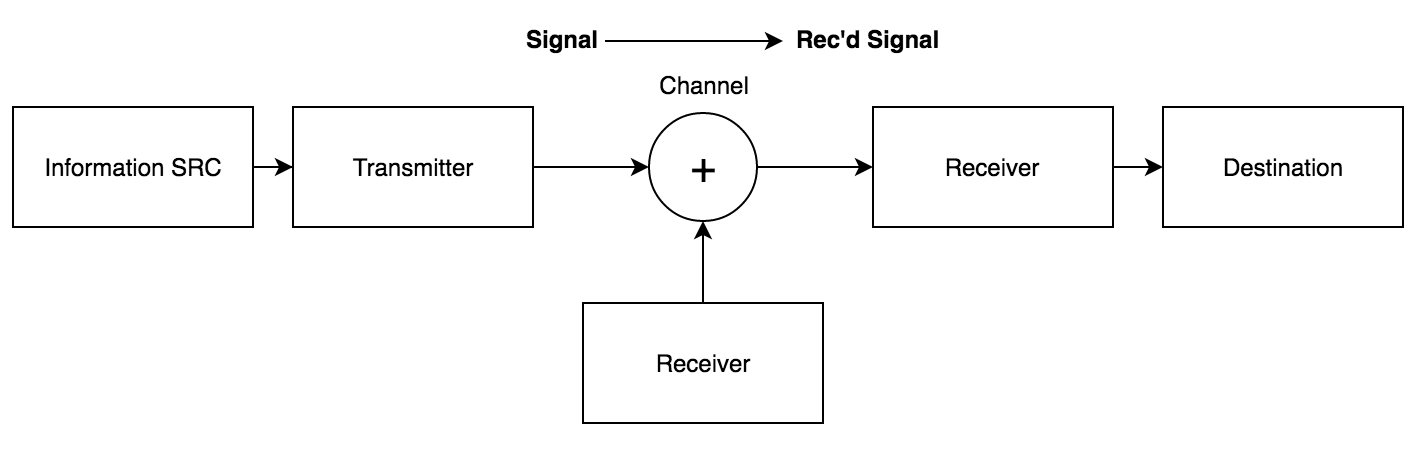
\includegraphics[scale=0.5]{pipeline}
\end{figure}
Information may be conveyed in multiple ways; for example, by a person talking, a video, or pictures. Our goal is to model this kind of information as a system with one output and no input. The information is therefore a box that emits output probabilistically, and we will therefore be spending 1-2 weeks on probability, specifically regarding distribution functions and expectation. This is illustrated in the ``information source'' box---the job of the information source is to \textbf{provide the signal}. 

We will next define the compression problem; having obtained numbers as a stream, the problem is to remove the redundancy in a stream. In particular, we will discuss both lossless and lossy compression. One of the most critical ideas in this course is that of entropy, and we will define the concept (in general, a notion of how much information is originating from the source). We will also discuss the sensibility of such a definition and potentially expand upon it. An overarching concept here will be our definition of the performance of a compression algorithm via the source compression theorem and the boundedness of compression algorithms. This is illustrated in the ``transmitter'' box---the job of the transmitter is to \textbf{remove all redundancy}.

We will subsequently discuss the channel circle, which we will model with conditional probability distribution functions (PDFs). The output of this box, the receiver signal, is input to the receiver box, which has the job of \textbf{reconstruction of the signal and the noise}; this is known as the coding problem. Much like the compression problem of the source, the channel has the capacity problem (how much information can be transmitted?). And similar to the compression theorem, we will discuss the channel coding theorem, which will help us determine which parts of a code will require more redundancy for transmission. 

We will finally discuss Shannon's theorem, in which he states that a communication with no loss and arbitrary cost (due to a constraint on the amount of bandwith, power, etc.) is possible if the entropy of the source $H$ is less than the capacity of the channel $C$. In our course, we will first discuss the pipeline for lossless compression and then move to lossy compression.

\section{August 24, 2016}
Knowing what a random variable is and what it means is important for the source to transmitter relationship. 
\subsection{Random Variables}
\definition A random variable is a real-valued function of the outcome of an experiment. By definition, it is not deterministic.
\notation We will represent random variables with capital letters (for example, $X, Y, Z$).
\example[What are Random Variables?] (a) A coin is tossed ten times. Determine the number of heads obtained from the coin toss. The number of heads is the random variable in this case. (b) Given two rolls of die, identify their sum (a random variable) and the second roll raised to the fifth power (another random variable). (c) The time to transmit a message, the delay with which a message is received, and the number of errors in a message are both themselves random variables. \\

\noindent Two types of random variables exist; discrete variables and continuous variables. 
\definition[Discrete RV] A discrete random variable is one that has a finite set of outcomes (or is countably infinite), and has a probability associated with each outcome. 
\definition[Continuous RV] A continuous random variable is one that has a non-finite, uncountable set of outcomes. 

\example Define the function 
\begin{equation*}
sgn(a) = \begin{cases}
1 &a > 0\\
0 & a = 0 \\
-1 & a < 0
\end{cases}
\end{equation*}
The variable $a$ is a continuous random variable, while $sgn(a)$ is a discrete function (with outputs $\in \{1, 0, -1\}$)
\subsubsection{Probability Mass Function (pmf)}
Probability mass functions are functions of a discrete random variable, describing all instances of a random variable occurring and its associated probabilities. Define $X$ as a random variable, and write $P(X = x)$ as $p_X(x)$. Then $\sum_x p_X(x) = 1$. Consider two tosses of a coin, letting $X$ equal the number of heads obtained. We therefore have 
\begin{equation*}
p_X(x) = \begin{cases}
1/4 & x =0\\
1/2 & x=1\\
1/4 & x=2 \\
\end{cases}
\end{equation*}
note that $p_X(x)$ is clearly a discrete function that takes on values $x \in \{0, 1, 2 \}$ with respective output probabilities. 
\subsubsection{Probability Density Function (pdf)}
%\begin{figure*}[h]
%\centering
%    \begin{tikzpicture}
%    \path[draw](0,0)--(0,5);
%    \path[draw](0,0)--(5,0);
%     \path[draw] (0,0) -- (2,2) -- (4,0);
%    \end{tikzpicture}
%\end{figure*}
Probability density functions are functions of a continuous random variable. Define $X$ as a random variable. In this case, the expression $P(X = x)$ is meaningless (in fact, it is defined as 0). The probability of a range of values from $x = a$ to $x = b$ is more relevant; in particular, $\int_{-\infty}^{\infty}p_X(x) = 1$. 

\example Edgar's driving time to school is between 15 and 20 minutes if it is sunny and between 20 and 25 minutes if it is a rainy day. Assume a day is sunny with $2/3$ probability and rainy with $1/3$ probability. Construct the respective PDF. \\

\noindent The PDF construction is quite simple; remember that $\int_{-\infty}^{\infty}p_X(x) = 1$. 
\begin{equation*}
p_X(x) = \begin{cases}
2/15 & 15 \leq x \leq 20\\
1/15 & 20 \leq x \leq 25 \\
0 & x \geq 25 \\
\end{cases}
\end{equation*}

\subsubsection{Types of Random Variables}
We will define these distributions in terms of a coin toss. 

\xhdr{Bernoulli (Discrete)} Toss a coin, and it define the probability of heads as $p$. The respective PMF is 
\begin{equation*}
p_X(x) = \begin{cases}
p & x = 1\\
(1-p) & x = 0
\end{cases}
\end{equation*}

\xhdr{Binomial (Discrete)} Toss a coin $N$ times, and define $x$ as the number of heads obtained in $N$ tosses. Let $N = 10$, and define the probability of heads as $p$. Then the respective PMF is 
\begin{equation*}
p_X(x) = \begin{cases}
(1-p)^{10} & x = 0\\
{10 \choose 2}p^2(1-p)^8 & x = 2 \\
\dots & $other values of $ x \in [0, 10] \cap \mathbb{N}
\end{cases}
\end{equation*}

\xhdr{Geometric (Discrete)}  Repeatedly toss a coin until the first ``success.'' This means that we may theoretically have countably infinite $P(X = 1), P(X = 2), P(X = 3), \dots$ output values. Define success to be a head, and the probability of heads as $p$. Then, we have
\begin{equation*}
p_X(x) = \begin{cases}
p & x = 1\\
(1-p)p & x = 2 \\ 
(1-p)^2p & x = 3 \\
\dots & $other values of $ x
\end{cases}
\end{equation*}

\xhdr{Poisson (Discrete, $\sim$ Binomial)} Instead of tossing a biased coin and counting the number of heads (a binomial distribution), count the number of times one must replace a biased lightbulb in a time $t$ (with the lightbulb being on or off). This makes the poisson distribution a discrete one. Our distribution function is 
\begin{equation*}
p_X(x) = \frac{e^{-\lambda} \lambda^x}{x!}
\end{equation*}
where $\lambda$ is an arbitrary constant. The number of decay events in some radioactive element, for example, may be modeled using a Poisson distribution. Anything that involves units of time and something happening within a period of time $t$ may include a Poisson distribution. 

\xhdr{Exponential (Continuous, $\sim$ Geometric)} Given a biased lightbulb, identify the amount of time until the bulb burns out. Examples of the use of this function include rates (as opposed to numbers defined with the Poisson distribution). The PDF is defined as
\begin{equation*}
p_X(x) = \begin{cases}
\lambda e^{-\lambda x} & x \geq 0 \\
0 & $otherwise$
\end{cases}
\end{equation*}
where $\lambda$ is an arbitrary constant.

\xhdr{Gaussian (Continuous)} If one does enough experiments of a binomial random variable, the distribution will end up looking like a Gaussian. The PDF is
\begin{equation*}
p_X(x) = \frac{1}{\sqrt{2\pi\sigma^2}}e^{\frac{-(x - \mu)^2}{2\sigma^2}}
\end{equation*}
where $\mu$ and $\sigma$ are parameters that can be treated as constants. 
\section{August 26, 2016}
\subsection{Properties of Random Variables}
We will be defining expectation and variance, and deriving equations regarding these properties of random variables. 
\subsubsection{Expectation (Mean) of a Random Variable}

\xhdr{Discrete} The notation is $E[X]$, where $X$ is the random variable. We have $$E[X] = \mu = \sum_x x_i p(x_i)$$For example, the expected value of rolling a die is 3.5. 

\xhdr{Continuous} The notation is again $E[X]$, where $X$ is the random variable. We have $$E[X] = \mu = \int_{-\infty}^\infty x p(x) dx$$

\noindent In fact, it is possible to find the expected value of any function of a random variable. For example, $$E[X^2] = \sum_x x_i^2 p(x_i)$$ $E[X]$ is called the ``first moment'' of a variable, and $E[X^2]$ is called the ``second moment.''

\subsubsection{Variance of a Random Variable}

We will denote the variance of a random variable as $V[X]$ (in class, this is denoted $Var[X]$). The variance depends on the expectation, and is written as $$V[X] = E[(X - E[X])^2] = E[X^2] - E[X]^2$$It is possible to expand this condensed form in both discrete and continuous forms. 

\xhdr{Discrete} $V[X] = \sum_x(x_i - \mu)^2p(x_i)$
\xhdr{Continuous} $V[X] = \int_{-\infty}^\infty (x_i - \mu)^2 p(x_i)dx$

\noindent The variance is always a positive quantity, and the standard deviation $\sigma = \sqrt{V[X]}$.

\subsubsection{The Mean and Variance of a Bernoulli Distribution}
Recall the definition of a Bernoulli random variable,
\begin{equation*}
p_X(x) = \begin{cases}
p & x = 1\\
(1-p) & x = 0
\end{cases}
\end{equation*}
We can write 
\begin{align*}
E[X] &= \sum_x x_i p(x_i) \\
&= 1(p) + 0(1-p) \\
&= p
\end{align*} 
The variance is defined as $E[(x-\mu)^2]$, so we have
\begin{align*}
V[X] &= \sum_x (x_i - p)^2 p(x_i) \\
&= (1-p)^2 p + (0-p)^2 (1-p) \\
&= p(1-p)
\end{align*}

\subsubsection{The Mean and Variance of a Geometric Distribution}
Recall the definition of a geometric random variable,
\begin{equation*}
p_X(x) = \begin{cases}
p & x = 1\\
(1-p)p & x = 2 \\ 
(1-p)^2p & x = 3 \\
\dots & $other values of $ x
\end{cases}
\end{equation*}
We can write %(todo: clean the tex up)
\begin{align*}
E[X] &= p(1-p)^0 + 2p(1-p)^1 + \dots \\
&= p(1-p)^0 + p(1-p)^1 + p(1-p)^2 + \dots = 1 \\
&\qquad \qquad \: \: \: \: \: \: + p(1-p)^1 + p(1-p)^2 + \dots = 1-p \\
& \qquad \qquad \qquad \qquad \qquad \: \: + p(1-p)^2 + \dots = (1-p)^2
\end{align*}
The critical insight here is that $2p(1-p)$ can be written as $p(1-p) + p(1-p)$, and $3p(1-p)^2$ can be written the same way, with each sub-series forming a geometric series. We then sum the resulting geometric series $1 + (1-p) + (1-p)^2 + \dots$, yielding $E[X] = \frac{1}{p}$. \\

\noindent The variance is defined as $V[X] = E[X^2] - E[X]^2$, which simplifies (after much algebra) to $$V[X] = \frac{1-p}{p^2}$$

\subsubsection{The Mean and Variance of a Binomial Distribution}
Recall the definition of a binomial random variable,
\begin{equation*}
p_X(x) = \begin{cases}
(1-p)^{10} & x = 0\\
{10 \choose 2}p^2(1-p)^8 & x = 2 \\
\dots & $other values of $ x \in [0, 10] \cap \mathbb{N}
\end{cases}
\end{equation*}
We can write
\begin{align*}
E[X] &= \sum_x x_i p(x_i) \\
&= 0p(0) + 1p(1) + 2p(2) + \dots \\
&= 1\left(p(1-p)^{n-1} {n \choose 1}\right) + 2 \left(p^2(1-p)^{n-2} {n \choose 2} \right) + \dots \\
&=  np \left({n-1 \choose 0} (1-p)^{n-1} + {n-1 \choose 1} p(1-p)^{n-2} + {n-1 \choose n-1}p^{n-1}\right) \\
&= np((p+1)-p)^{n-1} \\
&= np
\end{align*}

\noindent Note that a binomial random variable is really just a bunch of independent binomial random variables added up. So we can sum the variances to obtain $V[X] = np(1-p)$. In retrospect, we could have done the same for $E[X]$.

\section{August 30, 2016}

\subsection{Wrapping up Means and Variances} 

Recall the following facts from last time. Bernoulli: $E[X] = p$, $V[X] = p(1-p)$. Binomial: $E[X] = np$, $V[X] = np(1-p)$. Geometric: $E[X] = 1/p$, $V[X] = (1-p)/p^2$. 

\subsubsection{The Mean and Variance of a Poisson Distribution}
We may go over this in the future. For now, note that $E[X] = V[X] = \lambda$. 

\subsubsection{The Mean and Variance of a Exponential Distribution}
Here, we have $E[X] = 1/\lambda$ and $V[X] = 1/\lambda^2$. The derivation for $E[X]$ is as follows, noting that $p(x) = \lambda e^{-\lambda x}$. So,
\begin{align*}
E[X] &= \int_{0}^{+\infty} x \lambda e^{-\lambda x} dx \\
	&= \lambda \left[ \frac{-x}{\lambda} e^{-\lambda x} \bigg|_0^\infty+ \frac{1}{\lambda} \int_0^{+\infty}e^{-\lambda x}dx \right] \\
	&= 0 + \left(\frac{-1}{\lambda} \right)e^{-\lambda x}\bigg|_0^\infty \\
	&= \frac{1}{\lambda}
\end{align*}

\subsubsection{The Mean and Variance of a Gaussian Distribution}
Remember that the PDF is
\begin{equation*}
p_X(x) = \frac{1}{\sqrt{2\pi\sigma^2}}e^{\frac{-(x - \mu)^2}{2\sigma^2}}
\end{equation*}
where $\mu$ and $\sigma$ are parameters that can be treated as constants. The integration involves the error function, and yields $E[X] = \mu$ and $V[X] = \sigma^2$. 

\subsection{Linearity of Expectation}
The central idea is that, if one has properties of random variables $X$ and $Y$, it would be nice to also know properties about the sum $X + Y$. 

\theorem[Linearity of Expectation] $E[X + Y] = E[X] + E[Y]$.
\begin{proof}
This statement is the same as $$\sum_x \sum_y (x + y)p(X = x, Y = y)$$where the probability function is certainly not conditional, but may not be represented as the product of both individual probabilities as no assumptions are made of independence. This may be rewritten as $$\sum_x \sum_y x p(X = x, Y = y) + \sum_x \sum_y y p(X = x, Y = y)$$which is equivalent to $$\sum_x x \sum_y p(X =x, Y = y) + \sum_y \sum_x y p(X =x, Y = y)$$Note that, in the left sum indexed by $y$, the probabilities of $y$ sum to 1 so the resulting value is simply $p(X = x)$. The same is true for the right sum, yielding $$\sum_x xp(X =x) + \sum_y y p(Y = y)$$which completes the proof. 
\end{proof}
\noindent Note that this result is not true for the variances; i.e.  $V[X+Y] = V[X] + V[Y]$. The linearity of variances is only true when $X$ and $Y$ are independent (really, uncorrelated). 

\example{Let $Y = aX + b$}. We have $E[Y] = aE[X] + b$. The linear shift does not affect variance, and so our resulting variance is $V[Y] = a^2V[X]$. 

\example{You have an urn with three types of balls: 8 blue, 4 white, and 2 orange. Choose two balls at random. You win two dollars for every blue ball, lose one dollar for every white ball, and are not changed by an orange ball. Determine all values of $X$, your winnings, the probability of $X$, and $E[X]$.} \\

\noindent A listing of possible winnings is as follows: 4, 2, 1, 0, -1, -2. $P(4) = \binom{8}{2}/\binom{14}{2}$. $P(2) = \binom{8}{1} \binom{2}{1} / \binom{14}{2}$. $P(1) = \binom{8}{1} \binom{4}{1} / \binom{14}{2}$. $P(0) = \binom{2}{2} / \binom{14}{2}$. $P(-1) = \binom{2}{1} \binom{4}{1} / \binom{14}{2}$. $P(-2) = \binom{4}{2} / \binom{14}{2}$. Multiply each value with its probability to obtain $E[X] = 12/7 \approx 1.71$.

\example One of the numbers $(1-10)$ is randomly chosen. You are to try to guess the number by asking yes or no questions. Compute the expected number of questions if (a) your ith question is ``is it $i$?'', and (b) with each question, you try to eliminate $1/2$ of the remaining as nearly as possible. \\

\noindent (a) The expected value is $$E[X] = \frac{1}{10} \cdot 1 + \frac{1}{10} \cdot 2 + \frac{1}{10} \cdot 3 + \cdots = 5.5$$ 

\noindent (b) Draw a decision tree (for example, first split has left branch $1,2,3,4,5$ and left branch has $6,7,8,9,10$). Count the probability for each number of moves and obtain $$E[X] = 4 \cdot \frac{4}{10} + 3 \cdot \frac{6}{10} = 3.4$$

\example Suppose that the average numbers of cars abandoned in a week on a certain highway is 2.2. Approximate the probability that there will be (a) no abandoned cars this week and (b) at least two abandoned cars in the next week. \\

\noindent (a) Use a Poisson distribution. $E[X] = \lambda = e^{-2.2}$. \\

\noindent (b) This is expressed as $1 - p_X(x = 1) - p_X(x = 0)$ which equals $1 - 2.2e^{-2.2} - e^{-2.2}$. 

\section{September 1, 2016}
This class was primarily reviewing Problemset 2. 
\theorem[Bayes] $P(A|B) \cdot P(B) = P(A \& B) = P(A \cap B) = P(B|A) \cdot P(A)$.

\section{September 6, 2016}
We will first go over some problems, and then talk more about information sources and whether it makes sense to model them as random variables. 
\subsection{Review Problems}
\example$X$ is a random variable with probability with probability distribution function. Let 
\begin{equation*}
f(x) = \begin{cases}
c(1-x^2) & -1 < x < 1\\
0 & x = $anything else$ \\
\end{cases}
\end{equation*}
(a) What is $c$? $\int f(x) dx = 1$, so we have $(cx - \frac{cx^3}{3}|_{-1}^1 = 1$, and $c = 3/4$. \\
(b) Recall the definition of $E[X] = \int xf(x) dx$. So, we have $E[X] = \int_{-1}^1 x (3/4) (1-x^2)dx = 0$. 

\example The PDF of lifetime of a certain type of electronic device is
\begin{equation*}
f(x) = \begin{cases}
10/x^2&  x > 10 \\
0 & x \leq 10 \\
\end{cases}
\end{equation*}
(a) What is $P(X > 20)$? Integrate from 20 to infinity and solve to obtain $1/2$. \\
(b) What is the probability that, of 6 such types of devices, at least three will function at least 15 hours? State assumptions. Assume that each case is independent. We have $P(X > 15) = 2/3$. So our expression for exactly 3 is $$1 - P(0) - P(1) - P(2)$$which equals $$1 - \binom{6}{0}(1/3)^6 - \binom{6}{1}(1/3)^5 (2/3) - \binom{6}{2} (1/3)^4 (2/3)^2$$

\example Find $E[X]$ of the following \\
(a) \begin{equation*}
f(x) = \begin{cases}
5/x^2&  x > 5 \\
0 & x \leq 5 \\
\end{cases}
\end{equation*}
(b) \begin{equation*}
f(x) = \begin{cases}
(x/4)e^{-x/2}&  x > 0 \\
0 & $otherwise$ \\
\end{cases}
\end{equation*}
(a) is 0, (b) is 4 (integrate by parts twice)

\subsection{Information Sources}

Can these sources be modeled as a system with no input and one output and output emits symbols probabilistically?

\begin{table}[h]
\centering
\label{my-label}
\begin{tabular}{|l|l|l|l|l|}
\hline
\rowcolor[HTML]{EFEFEF} 
Type      & \begin{tabular}[c]{@{}l@{}}Source\\ (Black Box)\end{tabular} & Data                                                       & Characteristics of PDF                                                                   & Can you send less?                                                    \\ \hline
e-mail    & computer                                                     & text                                                       & frequency of letters, greetings, formatting                                              & Possible                                                              \\ \hline
telephone & receiver                                                     & sound                                                      & \begin{tabular}[c]{@{}l@{}}decibel range, tone, background noise, \\ pauses\end{tabular} & \begin{tabular}[c]{@{}l@{}}Possible\\ (similar to email)\end{tabular} \\ \hline
images    & camera                                                       & pixels                                                     & \begin{tabular}[c]{@{}l@{}}background, same pixel values for large\\ areas\end{tabular}  & Possible                                                              \\ \hline
video     & camera                                                       & \begin{tabular}[c]{@{}l@{}}series of\\ images\end{tabular} & stationary objects in video                                                              & Possible                                                              \\ \hline
\end{tabular}
\end{table}

\section{September 8, 2016 (Andrew)}
\subsection{Modeling English Probabilistically}
Today, we will go through the same thought experiment that Claude Shannon performed. Looking at English text, Shannon first analyzed whether it could be modeled probabilistically.

\xhdr{Zeroth Order} A simplistic zeroth order approximation involves assuming uniform distribution across all letters. This may be conducted by rolling a 27 sided die. A sample output might look like \textit{
XFOML RXKHRJFFJUJ ZLPWCFWKCYJ FFJEYVKCDSGHYD QPAAMKBZAACCIBZLHJQD}.

\xhdr{First Order} A first order approximation leverages the probabilities of certain letters. For example, $P_{X}(E) \approx 0.13$ and $P_{X}(W) \approx 0.02$. A sample output might look like \textit{OCRO HLI RGWR NMIELWIS EU LL NBNESBEYA THEEI}.

\xhdr{Second Order} A second order approximation utilizes the probability of a letter appearing given the preceding letter. A sample output might look like \textit{ON IE ANTSOUTINYS ARE T INCTORE ST BE S DEAMY ACAIW D ILONONASIVE}.

\xhdr{$n$th Order} We can extend this out to an $n$th order approximation, which uses information about the preceding $n-1$ letters to predict the value of the $n$th character. The larger the value of $n$, the more like English the model's output becomes. \\

\noindent Shannon assumed that all sources are {\bf ergodic}. Ergodic sources are those whose distributions do not change with time. While this may not hold true universally, it is a reasonable approximation for most practical applications of his work. 

\example The time (in hours) required to repair a machine is an exponentially distributed random variable with $\lambda = \frac{1}{2}$.\\
\noindent (a) What is P(repair time > 2hrs)? $P(X > 2) = 1 - \int_{0}^{2} \frac{1}{2} e^{-\frac{1}{2} x} dx$\\
\noindent (b) What is P(repair time > 10 | repair time > 9)? P(X > 10 | X > 9) = $\frac{P(X > 10)}{P(X > 9)}$ = $\frac{e^{-5}}{e^{-4.5}}$
\subsection{Memoryless Property}
A random variable is said to be {\bf memoryless} if information about the past does not have an impact on future results. For instance, in the case of Example 17 (b), the probability of waiting 10 hours given that you've waited 9 hours is equivalent to the probability of waiting for 1 hour. The exponential distribution is the only continuous random variable and geometric is the only discrete one. Formally stated:\\
$$P(X > m + n | X > n) = P(X > m)$$
\example Say that two people, Ms. Jones and Mr. Brown, are being serviced by two mail attendants whose time to completion is an exponential random variable. Mr. Smith is standing behind both. What is the probability that he will be the last person to leave the post office? 0.5 because the distribution is memoryless. 
\example The speed of a particle can be modeled with \begin{equation*} f(X) =	 \begin{cases}
								a x^2 e^{-b x^2} & x >= 0\\
								0 & x < 0
							\end{cases}
		\end{equation*}
		Where $b = \frac{m}{2kT}$. What value of a satisfies this pdf?\\
		$\int_{0}^{\infty} a x^2 e^{-b x^2} dx = \frac{\sqrt{\pi } a}{4 b^{3/2}} $\\
		$\frac{\sqrt{\pi } a}{4 b^{3/2}} = 1$\\
		$a = \frac{4 b^{3/2}}{\sqrt{\pi }}$
\example Given that $Z \sim N(0,1)$, and $g(x)$ is differentiable, prove that
$$E[g'(Z)] = E[Z * g(Z)]$$
We'll finish this example next time. 

\section{September 13, 2016}

Quick review of Bayes' theorem---we always have
\begin{align*}
P(A|B) &= \frac{P(A \& B)}{P(B)} \\
P(B|A) &= \frac{P(B \& A)}{P(A)} 
\end{align*}
If $A$ and $B$ are independent, $P(A \& B) = P(A) P(B)$, as $P(B | A) = P(B)$ and $P(A | B) = P(A)$. 

\subsection{Definition of Information} 
Our goal is to motivate the definition of a quantity called entropy. Consider a large stream of output. We are already convinced that this stream can be modeled as a random variable. Now, we will determine how much information is in the stream. 

\example[Motivation] Consider the letter ``q''. We are asked to guess the next letter; an obvious guess is ``u''. If we are told the letter is indeed ``u'', there is not much information gain (we are not very surprised). If, however, the letter is ``w'', significantly more information is revealed (and we are surprised as a result). We would therefore like to identify a function that can represent this idea. \\

\noindent In line with this idea, let's try different functions. $f(p) = 1/p$ and $f(p) = 1-p$ are both monotonically decreasing functions of $p$ that represent an increasing value with a decreasing probability. For a stream of letters, however, this becomes a problem. Additionally, we would like to think about this idea in terms of information (is there more or less information?). To resolve this issue, we will consider the concept of entropy.

\subsection{Entropy}

\definition[Entropy] Let $X$ be a random variable. $$H(X) = \sum_x p(x) \log \left( \frac{1}{p(x)} \right)$$ The entropy $H(X)$ represents the average amount of information of variable $X$. From this definition, it is easy to see that we have $f(p) = \log (1/p(x))$ which is actually quite similar to our initial discussion. Note that this is equivalent to $$E \left[ \log \frac{1}{p(x)} \right]$$which is why we refer to entropy as ``average information''. In both cases, the logarithm is base 2 as we refer to information in bits. 

\example What is the entropy of a fair coin?
\begin{align*}
H(X) &= \sum_x p(x) \log \left( \frac{1}{p(x)} \right) \\
&= \frac{1}{2} \log \frac{1}{1/2} + \frac{1}{2} \log \frac{1}{1/2} \\
&= 1
\end{align*}
\example What is the entropy of a biased coin? Note that we expect $H(X)$ to be smaller in this case as per our previous discussion. Let the coin have probability of heads $0.9$. 
\begin{align*}
H(X) &= \sum_x p(x) \log \left( \frac{1}{p(x)} \right) \\
&= \frac{1}{10} \log \frac{1}{1/10} + \frac{9}{10} \log \frac{1}{9/10} \\
&= 0.47
\end{align*}
\example What is the entropy of a biased coin with probability $p$? Note that we expect $H(X)$ to be smaller in this case as per our previous discussion. Let the coin have probability of heads $p$. 
\begin{align*}
H(X) &= \sum_x p(x) \log \left( \frac{1}{p(x)} \right) \\
&= p \log \frac{1}{p} + (1-p) \log \frac{1}{1-p} 
\end{align*}
As expected, this represents a parabola with $\frac{d H(X)}{dx} = 0$ at $x = 0.5$. One may plot this distribution on Mathematica with the command \texttt{Plot[-p Log[2, p] - (1 - p) Log[2, 1 - p], {p, 0, 1}]}.

\remark If all symbols occur with equal probability, $H(X)$ will simply be $\log m$ bits where $m$ is the number of possible values. Equivalently, $2^{H(X)} = m$ equally probable values. So, transmitting information only requires $m$ bits for each value $X$. 

\subsection{Quiz Review}

\example $X$ is a binomial random variable with expected value 6 and variance 2.4. Find $P\{X=5\}$.
\example Suppose two 4-sided dice have sides numbered 1-4. Let $X$ denote the sum of the dice. Find all values of $X$, the PMF of $X$, and $E[X]$.
\example $X$ is a random variable having possible values of 0 and 1 such that $P(X=0) = 2P(X=1)$. Find the PMF, expectation, and variance of $X$. 
\example A local soccer team has 5 more games to play. If it wins, they will play its final 4 games in upper bracket and win each game in this bracket is 0.4. If it plays in lower bracket, the probability of winning is 0.7. Given that the probability that it wins the game this weekend is 0.5, what is the probability that it wins at least 3 of its final 4 games?
\example Let pdf of $X$ be
\begin{equation*} f(X) =	 \begin{cases}
								a + b x^2 & 0 \leq x \leq 1\\
								0 & o/w
							\end{cases}
\end{equation*}

\noindent If $E[X] = \frac{3}{5}$, find $a$ and $b$. All solutions are left to the reader. 

\section{September 14, 2016}

Quiz today; no notes. 

\section{September 16, 2016}

Problemset for Thursday is seven problems on entropy. This is a strictly individual assignment, but collaboration is allowed so long as each student has a unique solution. 

\subsection{Review of Entropy}

We have so far defined the term ``entropy'' and done problems on fair and biased coin. With $m$ equally likely symbols, $H(X) = \log_2 m$ and $m = 2^{H(X)}$. 

\example The entropy of a fair six-sided die is simply $\log_2 6$. Know how to solve this problem with a biased die (different faces have different probabilities). 

\subsection{Properties of $H(X)$}

From our previous discussion, we have the following properties for $H(X)$
\begin{itemize}
\item $H(X) \geq 0$
\item $H_b(X) = (\log_b a) H_a(X)$, where $H_q(X)$ is $H(X)$ using a logarithm of base $q$ 
\item $H(X)$ does not depend on outcome, only on $p$'s
\item $E[X] \geq H(X)$
\end{itemize}

\noindent Note that ``nat'' (using the natural logarithm) is equivalent to $1/\ln 2$ bits. 

\example Let $X$ be a geometric random variable with $p = 1/2$. It is useful to know that
\begin{align*}
\sum_{n=1}^\infty r^n &= \frac{r}{1-r} \\
\sum_{n=1}^\infty nr^n &= \frac{r}{(1-r)^2}
\end{align*}
The solution is straight from the definition of entropy; the reader can confirm $H(X) = 2$.

\example Ask ``efficient'' questions of the form ``Is $X$ in the set $\mathcal{S}$'' to identify what the element $X$ is (think binary search), where $X$ is a geometric random variable with $p = 1/2$. Determine what your questions will look like, the expected number of questions, and the expected number of questions of $H(X)$.

By the memoryless property, it is equally likely that your guess will be correct or incorrect (if you say ``is $X$ 1'', the chance is $1/2$, and the chance of the rest is $1/2$. Similarly, if you say ``is $X$ 2?'', the chance is again $1/2$--there is no way to optimize this method). The expected number of questions $E[\text{Questions}] = \sum(\text{question \#})P(\text{question \#})$. So, we have $1(1/2) + 2(1/4) + 3(1/8) + \cdots$. We can follow the ``sum of sums'' approach delineated previously in the proof of the mean and variance of a geometric distribution to obtain $2$. As $2$ is also the entropy of such a geometric random variable, we are sure that this is the best method; this follows from $E[X] \geq H(X)$. 

\theorem[Jensen's Inequality] If $f$ is a concave up function ($f'' > 0$) on a given region and $a+b = 1$, we have $$af(x_1) + b f(x_2) \geq f(ax_1 + bx_2)$$Flip the inequality if $f$ is concave down ($f'' < 0$). A more general form of this is $$\sum c_i f(x_i) \geq f(\sum c_i x_i)$$where $\sum c_i = 1$. Again, flip the inequality if $f$ is concave down. 

\theorem Let $X$ assume values $\{x_1, x_2, x_3, x_4, \dots, x_r \}$. We may also denote this as ``let the PMF of $X$ be an $r$-dimensional vector $<p_1, p_2, \dots, p_r >$''. We have that (a) $0 \leq H(X) \leq \log r$, (b) $H(X) = 0$ if and only if $p_i = 1$ for some $i$, and (c) $H(X) = \log r$ if and only if $p_i = 1/r$ for all $i$. 

\begin{proof}
(a) Jensen's inequality allows us to write 
\begin{align*}
H(X) = \sum_x p(x) \log \left( \frac{1}{p(x)} \right) \leq \log \sum p_i (1/p_i) = \log r
\end{align*}
(b) If $p_i = 1$, all of the other probabilities must be zero. Therefore, $H(X) = \log 1 = 0.$
     To prove the inverted statement, use the idea that $p(x) \log{\frac{1}{p}}$ can never be negative. In fact, $p(x) \log{\frac{1}{p}}$ is only
     ever zero when $p=1$. Since every other p would produce a positive value for entropy, the only vector $p$ that will satisfy $H(X) = 0$ is 
     where one $p_i$ is 1 and the rest are 0. \\
     
\noindent (c) For the first part of the if and only if, $p_i = 1/r$, the operand of the sum can be taken out of the sum, simply leaving $\log r$. We can also write $2^{H(X)} = r$ which implies that there are $r$ equally likely outcomes. This necessitates that each outcome has probability $p_i = 1/r$. 
\end{proof}

\section{September 20, 2016}

\subsection{Differential Entropy}

We will discuss how to define entropy for continuous random variables. 

\theorem The differential entropy $h(x) = H_{\mathrm{diff}}(X) = h(f) = \int f(x) \log (1/f(x)) dx$. 

\begin{proof}

Define a random variable $X^{\Delta}$ with a pmf that has bins of arbitrary size $\Delta x$. If we define $x_i$ to be the event that $X$ is in bin $i$, we could write the entropy of $X^{\Delta}$ as 

\begin{align*}
H(X^{\Delta}) &= \sum_i P(x_i) \Delta x \log{\frac{1}{P(x_i) \Delta x}}  \\
H(X^{\Delta}) &= \sum_i P(x_i) \Delta x \log{\frac{1}{P(x_i)} } +  P(x_i) \Delta x \log{\frac{1}{\Delta x} } \\
H(X^{\Delta}) &= \sum_i P(x_i) \log{\frac{1}{P(x_i)} } \Delta x +  \sum_i P(x_i) \Delta x \log{\frac{1}{\Delta x} }
\end{align*}
Let $\Delta x \to 0$:
	$$H(X^{\Delta}) = \boxed{ \int f(x) \log{\frac{1}{f(x)}} dx} + \infty$$
	
\end{proof}
\noindent We define the quantity $\int f(x) \log{\frac{1}{f(x)}} dx$ to be the differential entropy of the pmf $f$. The quantity $\infty$ is referred to as the precision factor. From this, we determine that the total entropy of the variable increases as the measurements of the variable become more precise. 

\notation We write the differential entropy as either $h(X)$, $H_{\mathrm{diff}}(X)$, or $h(f)$. 
\subsection{Properties of Differential Entropy}
\theorem{If $Y = X + c$, $h(Y) = h(X)$}
\proof Left to the reader. 
\theorem{If $Y = cX$, $h(Y) = h(X)$ + $ \log{|c|}$}
\begin{proof}
Let $f$ be the distribution of $X$ and $g$ be the distribution of $Y$. Then $$h(Y) = \int g(y) \log \frac{1}{g(y)} dy$$With $y = cx$ and $dy = dx$, we can write the integral as $$h(Y) = \int c \: g(x) \log \frac{1}{g(cx)} dx$$But, since we have $g(cx) = f(x)/c$, this resolves to $$h(Y) = \int f(x) \log \frac{c}{f(x)} dx$$which is simply $h(X) + \log |c|$.
\end{proof}

\remark Note that, although Theorem 7 seems to indicate that more information is encoded with a simple multiplication by a constant factor, it turns out that the multiplication increases the number of bins, resulting in precision error. 

\subsubsection{Entropy of a Uniform Distribution}
\theorem{If $X \sim \mathcal{U}(0,  a)$, then the differential entropy $h(X) = \log{a}$}

\begin{proof}
We have $$h(X) = \int f(x) \log \left(\frac{1}{f(x)} \right) dx$$which can be simplified to $$\int_0^a \frac{1}{a} \log(a) dx = \log a$$
\end{proof}
\remark In the discrete case (and with $a \rightarrow 2a$ in the uniform distribution), if the number of outcomes is doubled, the entropy $H$ goes up by one bit. Note also that the entropy can be 0 or negative.
\begin{itemize}
\item if $a = 1, h(x) = 0$
\item if $a = 2, h(x) = 1$ (it takes one more bit than $\mathcal{U}(0, 1)$)
\item if $a = 1/2, h(x) = -1$ (it takes one less bit than $\mathcal{U}(0, 1)$)
\end{itemize}

\theorem Given a fixed lower bound and upper bound, no PDF can have a larger entropy than a uniform distribution. 

\begin{proof}
Heuristically, the probability density function on $\{x_1, x_2,..,.x_n\}$ with maximum entropy turns out to be the one that corresponds to the least amount of knowledge of $\{x_1, x_2,..,.x_n\}$, in other words the uniform distribution. For a more formal proof consider the following:

A probability density function on $\{x_1, x_2,..,.x_n\}$  is a set of nonnegative real numbers $p_1,...,p_n$ that add up to 1. Entropy is a continuous function of the $n$-tuples $(p_1,...,p_n)$, and these points lie in a compact subset of $\mathbb{R}^n$, so there is an $n$-tuple where entropy is maximized. We want to show this occurs at $(1/n,...,1/n)$ and nowhere else.

Suppose the $p_j$ are not all equal, say $p_1 < p_2$. (Clearly $n\neq 1$.) We will find a new probability density with higher entropy. It then follows, since entropy is maximized at
some $n$-tuple, that entropy is uniquely maximized at the $n$-tuple with $p_i = 1/n$ for all $i$. Since $p_1 < p_2$, for small positive $\varepsilon$ we have $p_1 + \varepsilon < p_2 -\varepsilon$. The entropy of $\{p_1 + \varepsilon, p_2 -\varepsilon,p_3,...,p_n\}$ minus the entropy of $\{p_1,p_2,p_3,...,p_n\}$ equals

$$-p_1\log\left(\frac{p_1+\varepsilon}{p_1}\right)-\varepsilon\log(p_1+\varepsilon)-p_2\log\left(\frac{p_2-\varepsilon}{p_2}\right)+\varepsilon\log(p_2-\varepsilon)$$
To complete the proof, we want to show this is positive for small enough $\varepsilon$. Rewrite the above equation as
$$-p_1\log\left(1+\frac{\varepsilon}{p_1}\right)-\varepsilon\left(\log p_1+\log\left(1+\frac{\varepsilon}{p_1}\right)\right)-p_2\log\left(1-\frac{\varepsilon}{p_2}\right)+\varepsilon\left(\log p_2+\log\left(1-\frac{\varepsilon}{p_2}\right)\right)$$

\noindent Recalling that $\log(1 + x) = x + O(x^2)$ for small $x$, the above equation is
$$-\varepsilon-\varepsilon\log p_1 + \varepsilon + \varepsilon \log p_2 + O(\varepsilon^2) = \varepsilon\log(p_2/p_1) + O(\varepsilon^2)$$
which is positive when $\varepsilon$ is small enough since $p_1 < p_2$.

\end{proof}
\subsubsection{Entropy of an Exponential Distribution}

\example Find $h(X)$ for the function 
\begin{equation*} f(x) =	 \begin{cases}
								\lambda e^{-\lambda x} & x \geq 0\\
								0 & x < 0 
							\end{cases}
\end{equation*}

\noindent It is easier to replace the $\log$ with a $\ln$ in the definition of entropy. Integrating by parts, we obtain $$h(X) = 1 + \ln \frac{1}{\lambda} = \ln \frac{e}{\lambda} = \log \frac{e}{\lambda} \text{ bits} $$

\theorem Given a random variable with mean $\mu$ and unconstrained otherwise, the exponential distribution achieves maximum entropy. Recall that the expected value for an exponential distribution is $1/\lambda$. 
\section{September 22, 2016}

As a review, we defined differential entropy as $$h(X) = \int f(x) \log \frac{1}{f(x)} dx$$and we discussed two distributions: the uniform distribution $\mathcal{U}(0, a)$ which has a differential entropy of $\log a$ bits and the exponential distribution which has a differential entropy $h	(X) = \log (\frac{e}{\lambda})$. 

\subsection{Entropy of a Gaussian Distribution}

\theorem $h(X)$ for the function 
\begin{equation*}
p_X(x) = \frac{1}{\sqrt{2\pi\sigma^2}}e^{\frac{-(x - \mu)^2}{2\sigma^2}}
\end{equation*}
where $\mu$ and $\sigma$ are parameters that can be treated as constants is $\frac{1}{2} \log 2 \pi e \sigma^2$.

\begin{proof}
We will start with the definition of entropy 
\begin{align*}
h(X) &= \frac{1}{\sigma \sqrt{2\pi}} \bigintss e^{\frac{-(x - \mu)^2}{2 \sigma^2}} \log \left( \frac{1}{\frac{1}{\sigma \sqrt{2 \pi}} e^{\frac{-(x - \mu)^2}{2 \sigma^2}}} \right) dx \\
 &=   \frac{-1}{\sigma \sqrt{2\pi}} \bigintss e^{\frac{-(x - \mu)^2}{2 \sigma^2}} \left[ \log \frac{1}{\sigma \sqrt{2\pi}} + \log e^{\frac{-(x - \mu)^2}{2 \sigma^2}} \right] dx
\end{align*}
The first additive term of the integral resolves to $\log \sigma \sqrt{2\pi}$ as it is simply the PDF (which integrates to 1). The second term is written as
\begin{align*}
\frac{1}{\sigma \sqrt{2\pi}} \bigintss e^{\frac{-(x - \mu)^2}{2 \sigma^2}} \cdot \frac{(x-\mu)^2}{2\sigma^2} dx
\end{align*}
which can be shown to resolve to the variance of $(x-\mu)$. Some algebra resolves this to $1/2$ in nats or $1/2\ln 2$ in bits. The overall entropy is therefore $\frac{1}{2} \log 2 \pi e \sigma^2$. 
\end{proof}
\section{September 26, 2016}

\subsection{Source Coding} 

We will be discussing source coding. Our goal is to remove redundancy from the source and code it ``efficiently'' and ``losslessly''. For the purposes of our discussion today, we will be using the English alphabet. 

\example Given the 26 letters of the English alphabet and their probabilities (assume letters are independent), find a way to encode the distribution (convert it into 0s and 1s) and decode the distribution (return it to the original state). If we decide to use 5 bits for each letter, it is easy to cover the entire alphabet (there are 32 combinations). 

\example Although the first encoding is acceptable, we would next like to associate the length of the code with the probability of the symbol. Given that the most probable letter is an ``E'', we can send a 0, and the second probable letter (``A'') can be encoded with a 1. The next letter, say ``T'', we can send 01, and so on. There is a problem here, however: we don't have a stop coding, so it is impossible to differentiate the end of a string and the start of another one. \\

\noindent Our general issue is that \textit{no code can be a prefix of another code}. Our two conditions are as follows:
\begin{itemize}  
\item \textit{Variable Length Codes.} Assign smaller codes to larger probability symbols
\item \textit{Prefix ``Free'' Codes.} No letter can be a prefix of another letter's code (instantaneous codes)
\end{itemize}
\remark A code is a prefix code if and only if it can be visualized with a tree. 

\example Consider the code mapping E $\rightarrow$ 0, T $\rightarrow$ 10, A $\rightarrow$ 110, and O $\rightarrow$ 111. This can certainly represented by a tree with binary splits, and therefore works with these four letters. 

\section{September 28, 2016}

\subsection{Huffman Coding}

As we discussed previously, our coding mechanism relies on two principles: frequent symbols have shorter code words and that our compression achieved is as close to the maximum entropy close to the entropy of the source (within 1 bit). \\

\noindent The Huffman coding algorithm can be written as follows.
\begin{itemize}
\item Find the two least probable symbols
\item Combine these symbols to make an imaginary composite symbol
\item Replace the two least probable symbols with the probability as the sum of the components
\item Repeat the process until you have 1 symbol left
\end{itemize}
\noindent The decoding process is written as 
\begin{itemize}
\item The code for each symbol is obtained by concatenating binary numbers that lead to a symbol
\item Each time two symbols are combined, two paths are labelled with a 1 (upper) and 0 (lower)
\item Wash, rinse, repeat. 
\end{itemize}
%\example 

\example The following details a sample Huffman encoding for sample $x_1 \dots x_6$. % (note that the last `1' is the probability; the coding starts on each branch). 
\begin{figure}[h]
\centering
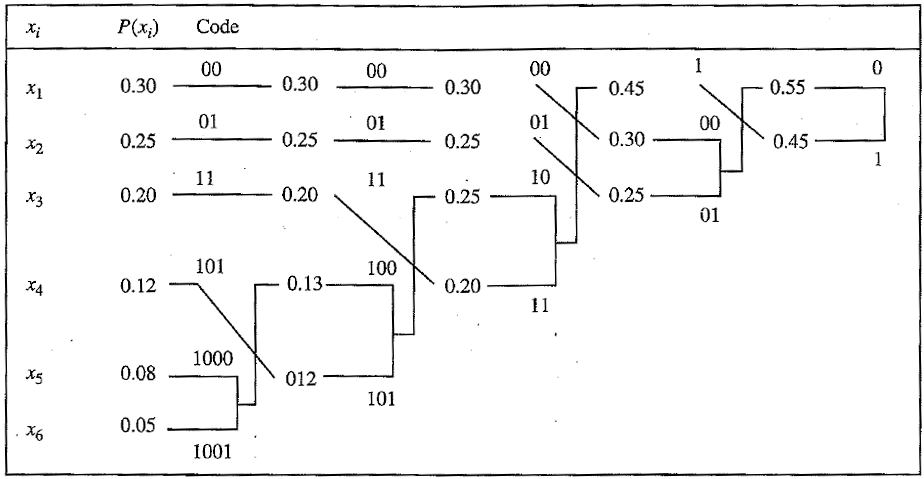
\includegraphics[scale=1.7]{huffman2.png}
\end{figure}

\example Given a list $X \in \{1,2,3,4,5\}$ with probabilities $\{0.25, 0.25, 0.2, 0.15, 0.15\}$. Identify the expected value of the length and the entropy $H(X)$. With the optimal Huffman code, $E[\text{Length}] = 2.3$ bits and $H(X) = 2.29$ bits. 

\example The Huffman code works for $n$-ary trees. In particular, the same example above with a ternary division yields $E[\text{Length}] = 1.5$ ternary digits. Ternary trees may require an ``additional'' value with probability 0 to balance the tree--insert this at the beginning to include it in overall computation. 

\example Which of these cannot be Huffman codes for any probability assignment? (a) $\{0, 10, 11\}$, (b) $\{00, 01, 10, 110\}$, (c) $\{01, 10\}$. (b) and (c) cannot be codes. 

\section{October 3, 2016}

\subsection{Lagrange Optimization}
Given a $f(x, y)$ or $f(x, y, z)$, we would like to determine the maximum and minimum of $f$ subject to a constraint $g(x, y)$ or $g(x, y, z)$.  We can write $$\mathcal{L}(x, y, z) = f - \lambda g$$of which we can find the critical points of $\mathcal{L}$ and determine whether those points are minima or maxima. (We'll discuss the intuition behind this later.) These critical points would be found by taking $\partial \mathcal{L} / \partial x, \partial \mathcal{L} / \partial y, \partial \mathcal{L} / \partial z, \partial \mathcal{L} / \partial \lambda$ and setting them equal to 0.   

\example[Lagrange]{Find the min and max values of $f(x, y, z) = x^2y^2z^2$ constrained by $x^2+y^2+z^2 = 1$.} We have 
\begin{align*}
f_x &= 2xy^2z^2 \\
f_y &= 2yx^2z^2 \\
f_z &= 2zx^2y^2
\end{align*}
and similarly $g_x = 2x$, $g_y = 2y$, and $g_z = 2z$. So, we have $f_x = \lambda g_x \implies 2xy^2z^2 = \lambda 2z$. We also have $f_y = \lambda g_y \implies 2yx^2z^2 = \lambda 2y$ and $f_z = \lambda 2z \implies 2zx^2y^2 = \lambda 2z$. Solving for lambda in each equation yields $\lambda = y^2z^2, \lambda = x^2z^2$, and $\lambda = y^2x^2$. These equations may be combined into the constraint (noting that $x^2 = y^2 = z^2$) so we have $3z^2 = 1$. So $z = \pm 1/\sqrt{3} = x = y$ for the maximum (where $f(x,y,z) = 1/27$). The minimum is obtained by setting one of $x, y$, or $z$ to 0 and the other two to fit the constraint (in which case $f(x, y,z) = 0$).  

\example $f(x,y) = xy^2$ on the circle $x^2 + y^2 = 1$. The solution is $x = \pm 1/\sqrt{3}$ and $y = \pm \sqrt{2}/\sqrt{3}$. These coordinates must be evaluated in $f$ to obtain minima and maxima. 

\example $f(x,y) = 3x + y$ constrained on $x^2 + y^2 = 10$. The solution is $x = \pm 3$ and $y = \pm 1$. Again, these coordinates must be evaluated to in $f$ to determine minima and maxima.

\subsection{Review of Huffman Coding}

Consider $X$ with PMF $\{1/21, 2/21, 3/21, 4/21, 5/21, 6/21\}$. Find the (a) binary and (b) ternary Huffman coding, and determine the lengths of each. (a) and (b) are left to the reader; the binary expected length is 2.42 and the ternary expected length is 1.62.

\section{October 5, 2016}
\subsection{Proof of Source Coding Theorem: Part 1 (LB: $H[X]$, UB: $H[X] + 1$)}
We will show that the expected length of an optimal prefix encoding $n$-ary tree is between $H[X]$ and $H[X] + 1$ (it has a lower bound of the entropy and the upper bound of (entropy + 1)).\footnote{Our proof will discuss binary trees, but it can be shown that it generalizes to an $n$-ary tree.} 

\lemma[Kraft Inequality] For any prefix code, the code word lengths $l_1, l_2, \dots, l_m$ must satisfy $$\sum_i 2^{-l_i}  < 1$$Conversely, given a set of code word lengths with this property, then there is a code with these lengths. 
\begin{proof}
For the first half of the Lemma, imagine a unit square. One may partition this square an arbitrary number of times, yet the area will remain constant ($2^{-l_i}$ is the area of a sub-square in the larger square). For the converse: given a set of code word lengths which satisfy Kraft, label the first node (lexicographically such that any `0' comes before any `1')\footnote{Here, `00' would come before `001'} of depth $l_1$ as code word 1. Remove all descendants from this node (so that no code is a prefix of another code) and label the first remaining node of depth $l_2$ as code word 2. Continuing this process will generate a prefix code with $l_1, l_2, \dots, l_m$. This is essentially a description of how to construct a prefix tree. 
\end{proof}

We have shown that any prefix code satisfies the Kraft inequality, and any code that satisfies the Kraft inequality is a prefix code. Our problem is now to find the prefix code with the minimum expected length.  This is equivalent to finding a set of lengths that satisfy the Kraft inequality and whose expected length $L = \sum p_i l_i$ is less than any other prefix code. We must therefore minimize $L  = \sum p_i l_i$ subject to the constraint $\sum 2^{-l_i} \leq 1$. We will neglect the integer constraint on $l_i$ and assume equality in the constraint. Following our method of Lagrange optimization, $$J = \sum p_i l_i + \lambda(\sum 2^{-l_i} -1)$$
Taking the partial with respect to $l_i$, we have $$\frac{\partial J}{\partial l_i} = p_i - \lambda 2^{- l_i} \ln 2$$because $\sum p_i l_i = p_1 l_1 + p_2 l_2 + \dots$ Setting the derivative equal to 0 yields $$2^{-l_i} = \frac{p_i}{\lambda \ln 2}$$which we may substitute into the constraint to find $\lambda$\footnote{The optimal code is achieved with equality.}.
\begin{align*}
\sum \frac{p_i}{\lambda \ln 2} &= 1 \\
\lambda &= \frac{1}{\ln 2}
\end{align*} 
We may then substitute this back into our original equation to obtain $p_i = 2^{- \l_i}$, so $l_i^* = -\log_2 p_i$. The optimal code (denoted with a $*$) is therefore $$L^* = \sum p_i l_i^* = -\sum p_i \log_2 p_i = H[X]$$In reality, $L^* \geq H[X]$. We have therefore proved the expected length $L^*$ is bounded below.  Since $\log_2 \frac{1}{p_i}$ may not be an integer, let $l_i = \ceil{\log_2 \frac{1}{p_i}}$. These lengths will still satsify Kraft since $$\sum 2^{-\ceil{\log_2 \frac{1}{p_i}}} \leq 2^{-\log \frac{1}{p_i}} = \sum p_i = 1$$This choice of code word lengths satisfies $\log_2 \frac{1}{p_i} \leq l_i \leq \log_2 \frac{1}{p_i} + 1$ due to the property of the ceiling. Multiplying by $p_i$ and summing over $i$, we get $$\sum p_i \log_2 \frac{1}{p_i} \leq p_i l_i < \sum \left[p_i \log_2 \frac{1}{p_i}\right] + \sum p_i$$Analogously, $H[X] \leq L < H[X] + 1$. Since $L \geq L^*$, $H[X] \leq L^* < H[X] + 1$. 

\section{October 7, 2016}

There are certainly many optimal codes, of which we will prove Huffman is one. 

\subsection{Proof of Source Coding Theorem: Part 2 (Optimality of Huffman)}

Before we can show that Huffman is optimal, we must prove some properties of a particular optimal code. 

\lemma For any distribution, there exists an optimal prefix code with a minimum expected length that satisfies the following:
\begin{itemize}
\item If $p_j > p_k$, then $l_j \leq l_k$ ($p$ denotes probability, $l$ denotes length)
\item Two largest code words code words have the same length
\item Two longest code words differ only in the last bit and correspond to the least likely symbols
\end{itemize} 

\begin{proof}
The proof really amounts to swapping, trimming, and rearranging code words. Consider an optimal code $C_m$ with $m$ symbols. Assume that $p_1 \geq p_2 \geq p_3 \geq \dots \geq p_m$. As the code is optimal, $\sum_i p_i l_i$ is minimal (as close to $H[X]$ as possible, but certainly within the bounds $H[X]$ and $H[X] + 1$).

Consider a new code $C_m'$ with code words $j$ and $k$ of $C_m$ interchanged. The difference between the expected lengths of both code words $L(C_m') - L(C_m) = \sum p_i l_i' - \sum p_i l_i$ reduces to  $p_jl_k p_kl_j - p_jl_j - p_k l_k$, which equates to $(p_j - p_k)(l_k - l_j)$. By hypothesis, $(p_j - p_k) \geq 0$. Since this code is the ``best'' optimal code (as defined by the sum $\sum_i p_i l_i$ as minimal),  $L(C_m') - L(C_m) \geq 0$, and $l_k \geq l_i$. 

Next, if the 2 longest code words are not of the same length, then one can delete the last bit of the longest one and still satisfy the prefix property. 

Finally, if there is a maximum length code word without a sibling (a code that differs in the last bit), then we can delete the last bit of the code word and still satisfy the prefix property (similar to (b)). This reduces the expected length, contradicting the hypothesis that the prefix code has ``minimum expected length'' ($\sum p_i l_i$ is minimal). So, the two longest code words must differ only in the last bit---every maximum length code word in any optimal code has a sibling. 
\end{proof}

Given a code tree, we can (a) trim it, (b) change the order so that the word lengths are in increasing order (the shorter ones are on the top), and (c) swap the probabilities to lower expected length. The final state is known as the ``canonical form.'' Any tree can be converted to a canonical form by following this series of steps. 

\begin{figure}[h]
\centering
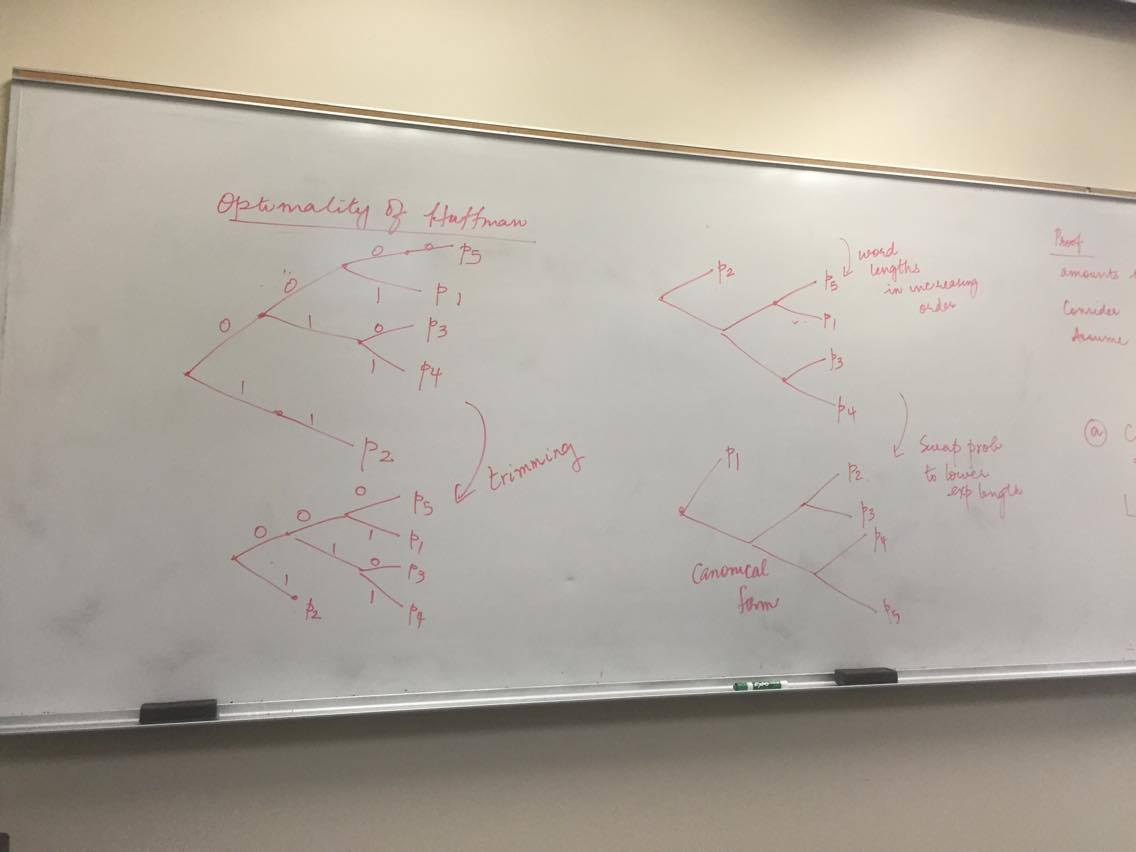
\includegraphics[width = \textwidth]{canonicalform.jpg}
\end{figure}
\theorem The Huffman encoding is a best optimal code (there exist other codes that achieve the same minimum length, but there is no better code). More precisely, if $C^*$ is Huffman coding and $C'$ is any other code, $L(C^*) \leq L(C')$. 
\begin{proof} We will show by induction that, if there is an optimal code at every level of the tree, then the tree is optimal. Define $C_m$ as the code for $\{p_1, p_2, \dots, p_m \}$ such that $p_1 \geq p_2 \geq \dots \geq p_m$. Define a merged code $C_{m-1}$ as a code obtained by taking the two longest code words and alloting them to a symbol with probability $p_{m-1} + p_m$. The original expected length of our tree is $$L(C_m) = \sum_{i = 1}^m p_i l_i$$This is equivalent to $$L(C_m) = \sum_{i-1}^{m-2} p_i l_i' + p_{m-1}(l'_{m-1} + 1) + p_m (l'_{m-1} + 1)$$where $l'$ is the length of the tree without the last two elements. The sum of the terms $p_{m-1}l'_{m-1}$ and $p_m l'_{m-1}$ are equivalent to $l'_{m-1}(p_{m-1} + p_m)$. This is just the merged code; we will define the last probability on the tree as $(p_{m-1} + p_m)$. We can write the resulting sum as $$\sum_{i = 1}^{m - 1}p_i' l_i' + p_{m-1} + p_m$$where we have the following definitions:

\begin{equation*}
l_i' = \begin{cases}
l_i &i \leq m-2\\
l_{m-1} & i = m-1\\
\end{cases}
\end{equation*} 
\begin{equation*}
p_i' = \begin{cases}
p_i &i \leq m-2\\
p_{m-1} + p_{m}& i = m-1\\
\end{cases}
\end{equation*}
The expected length is therefore equal to $$L(C_m) = L(C_{m-1}) + p_m + p_{m-1}$$So, minimizing $L(C_m)$ is equivalent to minimizing $L(C_{m-1})$. We have reduced the problem to one with $(m-1)$ symbols and a PMF $\{p_1, p_2, p_3, \dots, p_{m-2}, p_{m-1} + p_m \}$. We will now look for a code that satisfies the previous lemma and repeat the process until we have two symbols for which the solution is obvious. We have maintained optimality at every step of the tree, and since each level has been optimized, the entire tree has also been optimized. 
\end{proof}

\subsection{Huffman and 20 Questions}

\example Let $X_i = 1$ or $0$ if $i$-th object is good or defective, respectively. Let $X_i, X_2, \dots, X_n$ be independent with $\text{Pr} \{X_i = 1\} = p_i$. Also note that $p_1 > p_2 > \dots > p_n > 1/2$. The goal is to determine the set of all defective objects.  (a) Give a good lower bound on the minimum average number of questions. (b) Assuming worst case (that the longest sequence of questions is required), what is your last question? (c) Give a good upper bound on the expected number of questions required. 

(a) Treat each $X$ as a Bernoulli variable. Because each $X$ is independent, one can write the total entropy as the sum of the individual entropies. So, we have $H[X] = \sum_i H[X_i]$, where $H[X_i] = -[p_i \log p_i + (1-p_i) \log (1-p_i)]$. The good lower bound is this $H[X]$.

(b) ``Is $X_i$ defective for all $i$''

(c) The upper bound is just $H[X] + 1$. 

\section{October 11, 2016}

\subsection{Source Coding Examples}


\example[Huffman Codes with Costs] Words like Run! Help! and Fire! are short, not because they are frequently used, but perhaps because time is precious in the situations in which these words are required. Suppose that $X = i$ with probability $p_i$, $i = 1, 2, \dots, m$. Let $l_i$ be the number of binary symbols in the codeword associated with $X = i$, and let $c_i$ denote the cost per letter of the codeword when $X = i$. Thus the average cost $C$ of the description of $X$ is $C = \sum_{i=1}^m p_i c_i l_i$. 
(a) Minimize $C$ over all $l_1, l_2, \dots, l_m$ such that $\sum 2^{-l_i} \leq 1$. Ignore any implied integer constraints on $l_i$. Exhibit the minimizing $l_1^*,l_2^*, \dots, l_m^*$ and the associated minimum value $C^*$.
(b) How would you use the Huffman code procedure to minimize $C$ over all uniquely decodable codes? Let $C_{\text{Huffman}}$ denote this minimum.
(c) Show that $$C^* \leq C_{\text{Huffman}} \leq C^* + \sum_{i = 1}^m p_i c_i$$

\noindent Define $\sum_i p_i c_i$ as $K$. Our goal is to minimize $\sum_i p_i c_i l_i$ constrained by $\sum_i 2^{-l_i} \leq 1$. The Lagrange function is $\mathcal{L} = \sum_i p_i c_i l_i - \lambda(\sum 2^{-l_i} - 1)$. Differentiating $\mathcal{L}$ yields $\frac{\partial \mathcal{L}}{\partial l_i} = p_i c_i + \lambda 2^{-l_i} \ln 2$. We can then write 
\begin{align*}
p_ic_i &= -\lambda 2^{-l_i} \ln 2 \\
2^{-l_i} &= -\frac{p_i c_i}{\lambda \ln 2} \\
\sum_i 2^{-l_i} &= -\sum_i \frac{p_i c_i}{\lambda \ln 2} = -\frac{K}{\lambda \ln 2} \leq 1
\end{align*} 
Assuming the ideal case, we have $-\frac{K}{\lambda \ln 2} = 1$ so $\lambda = -\frac{K}{\ln 2}$. Then, $2^{-l_i} = \frac{p_i c_i}{\lambda \ln 2} = \frac{p_i c_i}{\frac{K}{\ln 2} \ln 2}$. Finally, we conclude that $l_i = -\log \left( \frac{p_ic_i}{K} \right)$. Our $C^* = \sum p_i c_i l_i$. Substituting the obtained value for $l_i$, we get $-\sum p_i c_i \log \left( \frac{p_i c_i}{K} \right)$. Noting that this equation looks quite similar to the form of entropy, we can multiply and divide by $K$ to obtain $$C^* = K \left( -\sum \frac{p_i c_i}{K} \log \left( \frac{p_i c_i}{K} \right) \right) = K H\left(\frac{p_i c_i}{K} \right)$$In the non-optimal case where $\log \left( \frac{p_i c_i}{K} \right) \neq \ceil{\log \left( \frac{p_i c_i}{K} \right)}$, we have $$\sum 2^{\ceil{\log \left( \frac{p_i c_i}{K} \right)}} \leq \sum 2^{\log \left( \frac{p_i c_i}{K} \right)} = 1$$by the property of the ceiling. This implies that $$\log \frac{p_i c_i}{K} \leq l_i \leq \log \frac{p_i c_i}{K} + 1$$which we may rewrite as $$\sum p_ic_i \log \frac{p_i c_i}{K} \leq \sum p_ic_i l_i \leq \sum p_ic_i \log \frac{p_i c_i}{K} + \sum p_ic_i$$So, we have $KH\left(\frac{p_ic_i}{K} \right) \leq C \leq KH\left(\frac{p_ic_i}{K} \right) + K$, and $$C^* \leq C \leq C^* + \sum_i p_i c_i$$

\example Random variable $X$ takes on six values $\{A, B, C, D, E, F\}$ with probabilities \\$\{0.5, 0.25, 0.1, 0.05, 0.05, 0.05\}$. (a) Construct a Huffman code for the random variable and find the expected length. (b) Construct a quaternary code and find its expected length. (c) One way to construct a binary code is to start with a quaternary code and then convert to binary (such that $a \rightarrow 00, b \rightarrow 01, c \rightarrow 10, d \rightarrow 11$). Find its average length. (d) Show that $\L_H \leq L_{QB} < L_H + 2$ where ``QB'' stands for quaternary-binary. 

Parts (a)--(c) are left to the reader. For part (d), $L_{QB} = 2L_{Q}$, and we know that $L_Q \leq H(X)_Q + 1$. $H(X)_Q = \sum_x \log_4 p(x) p(x) = \sum_x \frac{\log_2p(x)}{2} p(x)$. This evaluates to $0.5 \sum_x \log_2 p(x) p(x) = H(X)/2$. Therefore, $H(X)/2 \leq L_Q \leq H(X)/2 + 1$. So, $L_{QB} \leq H(X) + 2$, and $L_H \leq L_{QB}$ since $L_H$ is optimal. Since $H(X) \leq L_H$, $L_{QB} \leq L_H + 2$. 

\subsection{On Channels}
So far, we've looked at the source, which can be modeled as a random variable, and we showed that in order to code the source the best one can do is bounded by the entropy $H(X)$. (This is how much ``compression'' one can get out of a source.) We will now discuss the channel, which will morph the source output in some way. This morphing will also be modeled as a random variable but is conditioned on $X$, the random variable from the source. 

%\subsection{Conditional Probability}

%Problems are in the handout on Athena; this document will be updated once I can Ctrl+C, Ctrl+V

%\section{October 13, 2016}
%\example Imagine a party where everyone puts their hat into the center. Then, each person randomly takes a hat from the pool. What is the %probability that (a) there are no matches and (b) that there are exactly k matches. 

%We can represent the order in which the hats are drawn as a set of numbers, e.g. 4, 3, 2, 1 would mean that the first person draws hat four, the %second hat three, and so on. Observe the following pattern: 2, 1, 3, etc. Person 1 draws hat 2 and person 2 draws hat 1 forming a closed loop. %We refer to each such loop as a {\bf derangement} and call the total number of these derangements as $d_n$. 
%For instance, the probability of a $d_2$ derangement is equal to the probability that the first person does not draw their own hat times the %probability that the person whose hat is selected draws the first person's hat:
%$$d_2 = \frac{n - 1}{n} \times \frac{1}{n-1} = \frac{1}{n}$$
%Similar logic applies to 
%$$d_3 = \frac{n - 1}{n} \times \frac{n-2}{n-1} \times \frac{1}{n-2} = \frac{1}{n}$$. 
%
%---------------------------------------------------------------------------------------------------
\section{October 17, 2016 (Andrew)}
\subsection{Conditional Distributions}
We can make a conceptual mapping of standard distribution concepts onto conditional distribution concepts consider:
\begin{table}[h]
\centering
\begin{tabular}{|c|c|c|}
\hline
Function & Standard & Conditional\\
\hline
pmf & $P(X = x_0)$ & $P(Y|X = x_0)$\\
\hline
pdf & $f_X(x)$ & $f_{Y|X=x_0}(y|X=x_0)$\\
\hline
\end{tabular}
\end{table}
\example We have two R.V. $X$ and $Y$ such that $X\sim \mathrm{Poisson}(\lambda_1)$ and $Y\sim \mathrm{Poisson}(\lambda_2)$. What will the distribution of $X + Y$ be? It will a new poisson distribution. This property is NOT true in general of two independent RVs of the same distribution. It will hold for Poisson, Gaussian. 

\begin{proof}	Assume that $P(X = k) = \frac{e^{-\lambda_1} \lambda_1^k}{k!}$ and $P(Y = n) = \frac{e^{-\lambda_2} \lambda_2^n}{n!}$
		\begin{align*}
		P(X + Y = m)	&= \sum_{k=0}^m P(X=k) P(Y=m-k)\\
					&= \sum_{k=0}^m  \frac{e^{-\lambda_1} \lambda_1^k}{k!} \frac{e^{-\lambda_2} \lambda_2^n}{n!}\\
					&= e^{-(\lambda_1+\lambda_2)} \frac{1}{m!}\sum_{k=0}^m  \frac{m!}{k!(m-k)!}\lambda_1^k \lambda_2^{m-k}\\
					&= e^{-(\lambda_1+\lambda_2)} \frac{(\lambda_1 + \lambda_2)^m}{m!}
		\end{align*}\end{proof}
\example Given a continuous random variable $Z$ composed of two variables with pmf $f(x,y)$ such that 
\begin{equation*}
f(x,y) = \begin{cases}
\frac{12}{5} x(2-x-y) & 0 < x < 1, 0 < y < 1\\
0 & \text{otherwise}
\end{cases}
\end{equation*}
		what is $f(x|Y=y_0)$?
		Using an analogy of Bayes' Theorem:
			$$f_{x|Y=y_0}(x|Y=y_0) = \frac{f(x, y_0)}{f_Y(y_0)}$$
		We define $f_Y$ as the distribution of $Z$ exclusively with respect to $Y$. In other words, 
			\begin{align*}
			f_Y(y) &= \int_{-\infty}^{\infty}f(x,y)dx\\
				  &= \int_{0}^{1}\frac{12}{5} x (2 - x - y)dx\\
				  &= \frac{2}{5}(4 - 3 y)
			\end{align*}
		Substituting this value into our original equation we have that
			\begin{align*}
			f_{x|Y=y_0}(x|Y=y_0) &= \frac{\frac{12}{5} x (2 - x - y_0)}{\frac{2}{5}(4 - 3 y_0)}\\
					 &= \frac{6x (2 - x - y_0)}{4-3y_0}
			\end{align*}
This works because we are conditioning on \textit{one} instance of the variable $Y = y_0$.
\section{October 20, 2016}

\subsection{Continuing Conditional Distributions}

\example Suppose 3 balls are chosen without replacement from an urn consisting of 5 white and 8 red balls. Let $Y_i = 1$ if the $i$th white ball is drawn on the $i$th draw and $Y_i = 0$ otherwise. The $W$ balls are numbered. Find $P(Y_1, Y_2)$; this is easily done by drawing a table as follows:

% Please add the following required packages to your document preamble:
\begin{table}[h]
\centering
\begin{tabular}{@{}lll@{}}
\toprule
$Y_1$ & $Y_2$ & Probability                                                  \\ \midrule
0     & 0     & $\frac{1}{13} \times 1 + \frac{11}{13} \times \frac{11}{12}$ \\
0     & 1     & $\frac{11}{13} \times \frac{1}{12}$                          \\
1     & 0     & $\frac{1}{13} \times \frac{11}{12}$                          \\
1     & 1     & $\frac{1}{13} \times \frac{1}{12}$                           \\ \bottomrule
\end{tabular}
\end{table}

\noindent To find $P(Y_1 | Y_2 = 0)$, our sample space is constricted to the cases where $Y_2 = 0$. Our new distribution is $\frac{P(Y_1 = 0, Y_0 = 0)}{P(Y_2 = 0)}$ and $\frac{P(Y_1 = 1, Y_0 = 0)}{P(Y_2 = 0)}$ 

\example Verify that the following is indeed a joint pdf, and identify the difference between $f_{x|Y=y_0}(x|Y=y_0)$ and $f_x$, the density function of $X$.  \begin{equation*}
f(x,y) = \begin{cases}
\frac{6}{7} (x^2 + \frac{xy}{2}) & 0 < x < 1, 0 < y < 2\\
0 & \text{otherwise}
\end{cases}
\end{equation*}
(a) Evaluate the double integral $$\int_0^1 \int_0^2 \frac{6}{7} \left(x^2 + \frac{xy}{2}\right) \: dy \: dx = 1$$(b) $f_{x|Y=y_0}(x|Y=y_0) = \frac{f(x, y=y_0)}{\int_0^1 f(x, y=y_0) dx}$ and $f_x = \int f(x, y) dy$

\example $X$ and $Y$ are geometric random variables (independent) with the same parameter $p$. What do you think is $P(X = i | X + Y = n)$? Solution left to the reader. 

\subsection{Conditional Expectation} 

$E[X | Y = y_0]  = \sum_x x P(x | Y = y_0)$. Analogously, $\int x f_{X | Y = y_0} dx$. To compute expectation by conditioning, note that we can write \begin{align*} E[X] &= E_y[E[X | Y = y_0]] \\ &= \sum_y E[X | Y = y_0] P(Y = y_0) \end{align*}

\example Define \begin{equation*}
f(x,y) = \begin{cases}
\frac{e^{-x/y} e^{-y}}{y} & 0 < x < \infty, 0 < y < \infty \\
0 & \text{otherwise}
\end{cases}
\end{equation*}
Find $E[X | Y = y_0]$. The solution is $y_0$; details are left to the reader.  

\example Let the number of people who enter a store be a random variable with $\mu = 50$. The amount of money spent by each customer are independent random variables with $\mu = 8$. Suppose that the amount of money spent by each customer is independent of the total amount of money spent by all other customers who enter. Find the expected amount of money that the store makes in a day. 
Clearly the answer is 400, but we're going to write this formally. Let $N$ = the number of customers and $X_i$ = the amount spent by customer $i$. We wish to find $E[\sum X_i]$ which resolves to $E[E[\sum_{i = 1}^N X_i | N]]$. We will finish this next time. 

\section{October 24, 2016}

\subsection{Introduction and Examples of Channels}

Examples of channels include air, copper, fiber, and free space (satellites). The output sends a signal in as few bits as possible. The goal of the channel is to add redundancy in a smart way so one can efficiently decode the input. The channel recovers from the loss due to the input as best as possible. 

Consider a pipe with one end as the input and the other end as the output. Electron ``jiggling'' at one end results in (after a time delay) electron ``jiggling'' at the other end. Properties of the input include amplitude, frequency, and phase. When you get to the other side, the frequency remains the same, a delay exists (out of phase), and the amplitude decreases (in a phenomenon called attenuation). The attenuation and phase are characteristics of the medium. ``Jiggling'' the input with different frequencies has an unpredictable (nonlinear) relationship with the attenuation and phase, so these properties complicate the decoding process. 

From our initial terms, fiber tends to do the best with a minimal deviation in attenuation and phase given $\Delta$frequency. Another problem exists, however, with the consideration of \textit{noise}; that is, the superposition of outside mediums and the changing states of other jiggling molecules affect each molecule's jiggling. We claim (without proof) that noise is not predictable in any way, and at best one can come up with a probabilistic model (at worst, we can't do anything). 

\subsection{Modulation and De-modulation} 

Modulation is defined as the process of transforming binary digits to patterns. For example, 0 $\rightarrow$ send one pattern to analog signal  and 1 $\rightarrow$ send another pattern to analog signal. Each of these patterns is a signal of different frequency. Modulation is a ``perfect process''; it is always possible to convert these binary digits to signals. 

De-modulation (converting these signals into binary digits) is certainly not a perfect process due to the inclusion of noise (which might alter the modulated attenuation, phase, and frequency). 

This leads us to an input $X_1$ being transformed to an output $Y_1$ (we use different notation because $Y_1 \neq X_1$). We are hopeful that the output is truly $Y_1 = f(X_1)$ (some constant function of $X_1$), but it may be $Y_{2,3,\dots}$. This is where conditional probability is useful; given $X_1$, we are to determine $P(Y|X = x_1)$. Essentially, think of a channel as specifying $Y$ given each $X_i$. There exists a family of histograms/pdfs/pmfs, with one for each $X_i$. 

In investigating this concept, we will refine our definition of entropy and define the mutual information of two variables. 

\section{October 26, 2016}

\subsection{Mutual Information}

\begin{figure}[h]
\centering
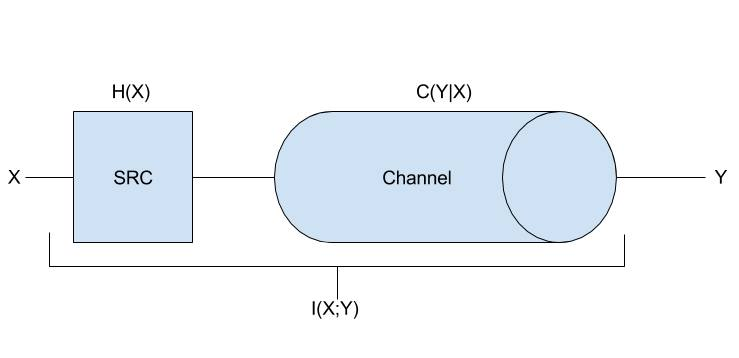
\includegraphics[scale=0.35]{sourcechannel}
\end{figure}

The source is defined as $H(X)$ which passes information to the channel. The output of the channel is $Y$ that changes based on the input to the channel, so we will model it as a conditional distribution. We will call this $C(Y | X)$ as it is conditioned on the input ($X$) and the output ($Y$). 

Let's look at this pipeline end-to-end. For a particular instance $Y_i$, the ``surprise value'' as we defined before in our discussion of entropy is $\log \frac{1}{P(Y_i)}$. Two factors contribute to this output: the input contribution and the noise contribution. The noise contribution can be written as $\log \frac{1}{P(Y_i | X_j)}$ ($i$ is the index of the particular output, and $j$ is the index of the particular input). The contribution due to the input is therefore $\log \frac{1}{P(Y_i)} - \log \frac{1}{P(Y_i | X_j)}$. For the overall contribution, we must average over all input/output pairs $x_j$ and $y_i$. This yields the mutual information of two random variables $X$ and $Y$. 

\definition[Mutual Information] $$I(X ; Y) = \sum_{x_i} \sum_{y_j} p(x_i, y_j) \log \frac{p(y_j | x_i)}{p(y_i)} = \sum_{x_i} \sum_{y_j} P(x_i, y_j) \log \frac{p(x,y)}{p(x)p(y)}$$
Note that $P(x_i, y_j)$ is a joint probability (the probability of seeing both $x_i$ and $y_j$). $I$ is the information contribution from the source to the channel. Our overall $$C(Y | X) = \text{max}_{\forall \text{sources}} I(X ; Y)$$that is, we seek to find the best source (that optimizes the mutual information). 

\subsection{Intuition of $C(Y | X)$, Part 1 (Picking the Channel from the Source)}

Given a fixed source, what is the best channel we can attach to this source? 

\definition[Distortion] The distortion $d(x_i, y_j) \geq 0$ with equality when $x_i = y_j$. Distortion characterizes how close or far the input is from the output. The average distortion is defined as $\overbar{d} = E_{X,Y}[d(x_i, y_i)]$

We will next define an algorithm to identify the input contribution of the source to the output. 
\definition We'd like to pick an optimized channel and define the source contribution of the output. Define this quantity as $H(X, \delta)$: 
\begin{itemize}
\item Pick an arbitrary average distortion $\delta$
\item Cannot tolerate a distortion of more than $\delta$, so only look at those channels where $\overbar{d} \leq \delta$
\item Of those channels, pick one of minimum $I(X;Y)$. (We're looking at the worst possible case.) 
\item That value of $I(X;Y) = H(X,\delta)$. 
\end{itemize}

\section{November 2, 2016}

\subsection{Guest Lecture: Joy Thomas}
We'll discuss practical data compression algorithms. Let $X \sim p(x)$ and $P(x = i) = p_i$. Then $H(X) = -\sum p_i \log p_i$. It turns out that $H$ is indeed related to the thermodynamic notion of entropy, but these relationships are not immediately obvious. If you have a code for $X$ called $C(X)$ that maps $X \rightarrow \text{some binary sequence}$, $E[L(X)] \geq H(X)$ and $E[L(X)] \leq H(X) + 1$. 

Real world data isn't independent or identically distributed. Assuming that the characters are independent is an approximation that isn't valid in practice; we can do better if we used blocks (compressing words as opposed to individual letters using an indexed dictionary). The notion of using a dictionary to compress has certainly been around for a while. 

\xhdr{Backwards Lookahead} Imagine the sequence $ABCAABBC \: | \: CAAB$. For every new character (between the two C's) we represent the characters by the offset since the last character seen. so in this case we would write the second set as 1, 5, 1, 5. We can represent this sequence in a unary code structure where the ceiling of log i  is 10. We can write 1110 for four bits  and then $i$ after that. The expected number of characters required to see a character is $1/p$ for that character. 

If we use this approach to compress the sequence, the expected length of the code is $\sum p(x) \log 1/p(x) + \sum p(x) \log \log 1/PM$. Another method is to construct the Huffman code for a distribution and use that to compress; however, this require two passes as opposed to the original one pass.   

\xhdr{LZ77} This is also known as the sliding window approach. Here, we transform the sequence $ABABABBBBAAABBB$ to $A, B, ABAB, BBB, A, AA, BBB$ (basically phrases that you've seen in the past). This becomes $(0, A), (0, B), (1, 2, 4), (1, 1, 3)$. It was proposed that LZ77 was the best possible by any finite state compressor (asymptotically). 

\xhdr{Find the Longest Match: LZ78} This requires a similar decoding as LZ77 with an expected length $\log p + \log A$. This algorithm achieved an optimal compression and is currently in use.

\subsection{Intuition of $C(Y | X)$, Part 1 (Picking the Channel from the Source) contd.}

The mutual information $I(X; Y) = \sum_{x_i} \sum_{y_j} P(x_i, y_j) \log \frac{P(y_j | x_i)}{P(y_i)}$. We are looking at the output of a channel as comprised of two parts: the noise part and the input contribution to the information we see in the output. We then discussed channel capacity, which is written as $C(Y|X) = \text{max over all sources} \: I(X;Y)$. We then revisited $H(X)$ to tie in this $I$ with our older definition of $H$. We defined the distortion $d(x_0, y_0) \geq 0$ with zero when $x_0 = y_0$. (Note that the average distortion $\bar{d} = E_{x,y}[d(x,y)]$.) We then picked an arbitrary distortion $\delta$ and only looked at channels that that have $\bar{d} \leq \delta$. Of those channels, pick the one with minimal $I(X;Y)$ that will allow for reconstruction with the distortion $\bar{d}_i \leq \delta$. That value of $I(X;Y)$ is $H(X)$ at that particular $\delta$. In particular, at $\delta = 0$, $\min I(X;Y) = I(X ; X) = H(X)$. With a greater distortion $\delta$ that is willing to be tolerated, $\min I(X;Y)$ (the amount of information that needs to be conveyed) decreases rapidly. 

Essentially, given a fixed source, we want to find a channel such that the minimum amount of distortion is required (so there is a minimum mutual information here). In the next part, we will fix the channel, and we want to maximize the amount of information that can pass through (so there is a maximum mutual information in Part 2). In all of our examples, we find $I(X;Y)$ given a fixed channel and try to maximize over the source distribution, mimicking Part 2. 

\subsection{Intuition of $C(Y|X)$, Part 2 (Picking the Source from the Channel)}

Now that we've covered the input to the channel, we will now consider the output side of the channel. Define a cost for sending information through the channel (limited bandwith for example). Let's call this cost function $b(x_0) \geq 0$, where $\bar{b} = E_x(b(x))$. Pick an arbitrary cost $\beta$ that you're willing to tolerate. We can't tolerate a cost greater than that $\beta$, so only look at sources where the average cost is less than or equal to that $\beta$. 

Of those channels, pick a source with maximum $I(X;Y)$. We then define $C(Y|X)$ as $$C(Y|X)_{\text{at a particular } \beta} = \max_{\forall \text{sources}} I(X;Y)$$
With a greater $\beta$ that can be tolerated, $\max I(X;Y)$ asymptotically reaches the channel capacity. So from Part 1, we have to put up with a certain distortion, and from Part 2 we have to also consider a certain cost. 
\section{November 3, 2016}

\subsection{Mutual Information Examples}

\example Noiseless binary channel with $0 \rightarrow 0$ (probability $p$) and $1 \rightarrow 1$ (probability $1-p$). We can write the channel capacity as $$p \log \frac{p}{p \times p} + (1-p) \log \frac{1-p}{(1-p) \times (1-p)}$$which is exactly the entropy!

\example Noisy channel with non-overlapping outputs such that $0 \rightarrow 1$ ($p = 1/2$), $0 \rightarrow 2$ ($p = 1/2$), $1 \rightarrow 3$ ($p = 1/3$) and $1 \rightarrow 4$ ($p = 2/3$). $p(0) = p$ and $p(1) = 1-p$. The mutual information again resolves to the entropy.

\example[Noisy Typewriter] The output is either received unchanged with probability 1/2 or transformed to the next letter with probability 1/2. The input has 26 symbols. We can write the mutual information as $$I(X;Y) = \frac{1}{2} p_A \log \frac{\frac{1}{2}p_A}{p_A\left(\frac{1}{2}p_A + \frac{1}{2}p_B\right)} + \dots $$This simplifies to $$\frac{1}{2}(p_A + p_B) \log \frac{1}{p_A + p_B} + \dots $$Setting $q_{AB} = \frac{p_A + p_B}{2}$ yields $$H(q_{AB}q_{BC}q_{CD}\dots) - 1$$to obtain the maximal distribution as uniform.

\example[Binary Symmetric Channel (BSC)] 

For this channel, we can write
$$ 
I(X; Y) = 2 \times \left[ \frac{1-p}{2} \log \left( \frac{1-p}{\frac{1-p}{2} + \frac{p}{2}} \right) + 
	      \frac{p}{2} \log \left( \frac{p}{\frac{1-p}{2} + \frac{p}{2}} \right) \right]
$$
which resolves to $H(p) - 1$.

\begin{figure}[ht]
\centering
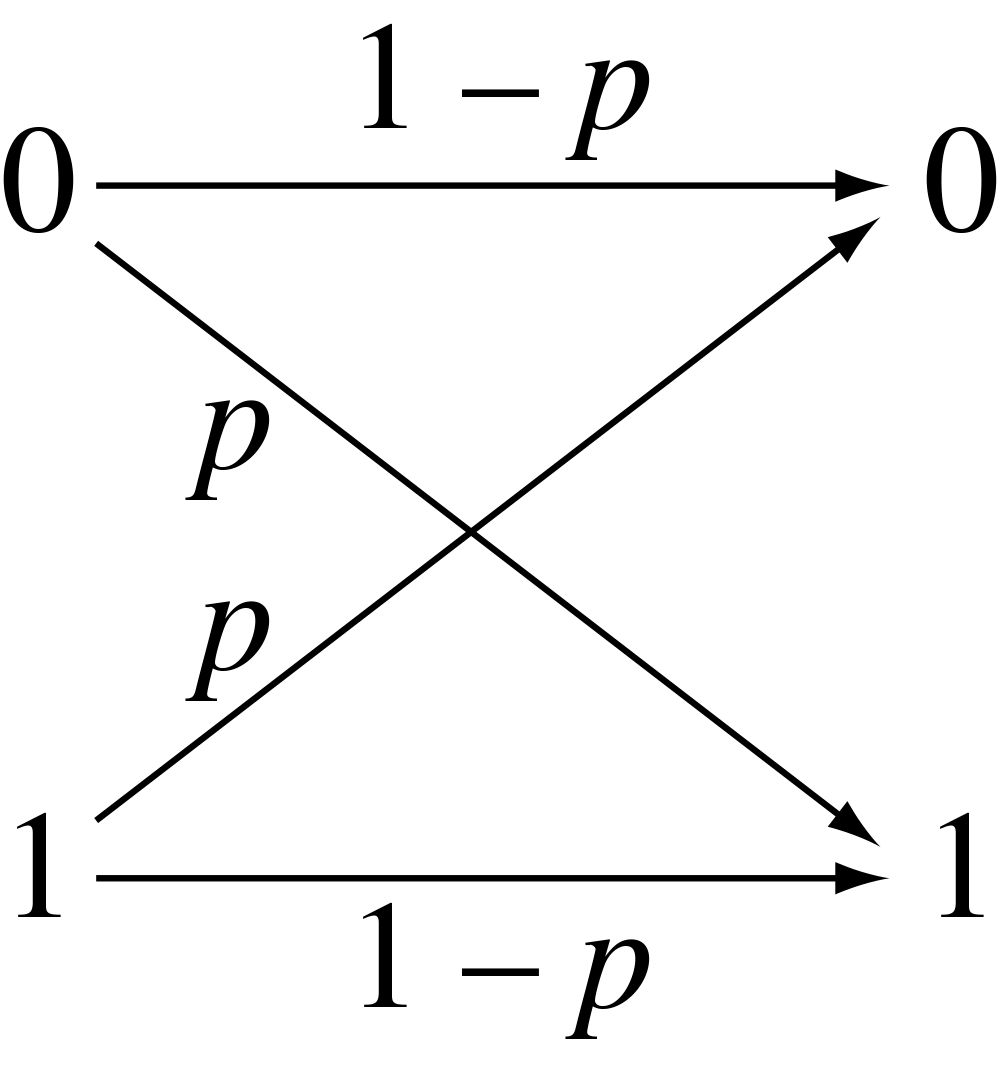
\includegraphics[scale=0.1]{binarysymmetric}
\end{figure}

\subsection{A Closer Look at $I(X;Y)$}

We have 
\begin{align*}
I(X;Y) = \sum \sum p(x_i, y_j) \log p(y_j | x_i) + \sum_x \sum_y p(x_i, y_j) \log \frac{1}{p(y_j)}
\end{align*}
The first term is defined as $-H(Y|X)$, the \textit{conditional entropy}, and the second is $H(Y)$. So it turns out that $I(X;Y) = H(Y) - H(Y|X)$. \\

\noindent A summary of important identities to be aware of:
\begin{itemize}
\item Conditional Entropy: $H(Y|X) = -\sum_x \sum_y f(x, y) \log f(y|x)$
\item Joint Entropy: $H(X, Y) = -\sum_x \sum_y f(x, y) \log f(x, y)$ (if $X$ and $Y$ are independent, $H(X, Y) = H(X) + H(Y)$)
\item $H(Y|X) = H(X, Y) - H(X)$
\item $I(X; Y) = H(Y) - H(Y|X) = H(X) - H(X|Y) = H(X) + H(Y) - H(X, Y)$
\end{itemize}

\section{November 8, 2016}
\example[Binary Erasure Channel] 

\begin{figure}[ht]
\centering
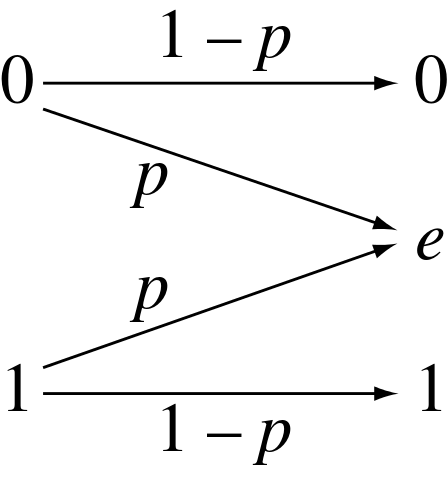
\includegraphics[scale=0.2]{binaryerasure}
\end{figure}

For this channel, we can write
$$
I(X; Y) = 2 \times \left[ \frac{1-p}{2} \log \left( \frac{1-p}{\frac{1-p}{2}} \right) \right] + 2 \times \left[ \frac{p}{2} \log \left( \frac{p}{p/2 + p/2} \right) \right]
$$
which resolves to $1-p$. 

\subsection{Gaussian Channel}
Given a channel with an input of some real number and an output of some real number + ``noise'' (which is defined as a gaussian real number distributed according to $N(0, \sigma^2)$. Assume that the input and noise are independent. We will attempt to find the best input distribution to maximize the capacity of this channel. 

\subsubsection{Part 1: Gaussian Source}

The output of the source is a single real number distributed according to $(\mu, \sigma_x^2)$. We are willing to tolerate a distortion $d(x,y)$ with an average distortion $\delta$. We therefore have $$h(X, \delta) = \frac{1}{2}\log(2\pi e \sigma^2) - \frac{1}{2} \log(2 \pi e \delta)$$in which the second term is obtained from the precision/distortion. 

\subsubsection{Part 2: Gaussian Channel}

Instead of having a distortion, here we have a cost for sending information through the channel. This cost is $\leq \beta$ and is related to the variance of the signal\footnote{This has to do with the voltage cost, which is left to the reader for further investigation}. So, we have $$\max_{\forall \text{sources}} I(X;Y) = h(Y) - h(Y|X)$$Let's call the noise $\eta$, which is factored in between the source $X$ and the output $Y$. We therefore have $$h(Y|X) = h(X+\eta | X) = h(\eta | X)$$as translation does not add any additional information (knowing $\eta$ is the same as knowing $X + \eta$)We can get rid of the $X$ as $\eta$ is independent of $X$, yielding $$h(Y|X) = h(\eta) = \frac{1}{2}\log(2\pi e \sigma^2)$$So we've determined that the second term in our definition for $I(X;Y)$ is $\frac{1}{2} \log (2 \pi e \sigma^2)$. For the first term, we know that $h(Y) = h(X+\eta)$. We know from a while ago that $V[Y] = E[Y^2] - E[Y]^2$. Assuming $E[Y] = 0$\footnote{Just accept it; apparently this doesn't matter anyway, but...} we can write $V[Y] = E[Y^2] = E[(X + \eta)^2]$. We can simplify this as \begin{align*}
E[Y^2] &= E[(X + \eta)^2] \\
	&= E[X^2 + 2X\eta + \eta^2] \\
	&= E[X^2] + 2E[X]E[\eta] + E[\eta^2] \\
	&= E[X^2] + E[\eta^2]
\end{align*}
because the noise has a mean of 0. We therefore have $E[Y^2] \leq \beta + \sigma^2$. Because there is an upper bound on the expected value $E[Y^2]$ and therefore on $V[Y]$, $Y$ being Gaussian maximizes $h(Y)$. Therefore, the maximum $I(X;Y) = h(Y) - h(Y|X)$ is obtained when $h(Y)$ is maximized (in Part 1 we bounded $H(Y|X)$) and $h(Y)$ is maximum when $Y$ is Gaussian. So $$\max I(X;Y) = \frac{1}{2}\log(2\pi e (\beta + \sigma^2)) - \frac{1}{2} \log (2 \pi e \sigma^2)$$We can simplify this as $\frac{1}{2} \log (1 + \frac{\beta}{\sigma^2})$ with constraint $\beta$ (the power constant), which is maximized when $X$ is also Gaussian. This expression defines the \textit{capacity} of a Gaussian channel. Note that this is true only because the noise is independent of the source; in particular, Gauss$_1$ + Gauss$_2$ = Gauss$_3$ if and only if Gauss$_1$ and Gauss$_2$ are independent. 

\subsection{Channel Codes: an Introduction}

Just as we defined entropy for the source and we talked about the entropy of various probability distributions, and then we moved onto coding entropy (notion of a tree + Huffman coding), here we will introduce channel codes (which are much more difficult than trees). Therefore, we'll be discussing circuits and digital representations next class. We'll introduce the concept of ``shift registers'' in the process. 

\section{November 10, 2016}

\subsection{Channel Codes}

The overall process is SRC $\rightarrow$ SE $\rightarrow$ CE (``bloats up'' the information enough for the noise) $\rightarrow$ noise $\rightarrow$ CD $\rightarrow$ SD.  

\xhdr{Channel Coder} Recall the source encoder/decoder diagram from earlier. The goal of the encoder is to eliminate all redundancy (I: source characters, O: bits). The goal of the decoder is to reconstruct the source characters (I: bits, O: reconstructed source characters). 

\xhdr{Channel Encoder/Decoder} The input of the channel encoder is bits, and it outputs a channel character stream (a pattern of jiggling electrons at one end of the wire). The channel encoder is between the source encoder and the source decoder. The goal of the channel encoder is to introduce controlled redundancy. The channel decoder has as input the noisy channel characters and (hopefully) outputs the reconstructed bits. 

\example[TDM] To convert bits in the channel encoder to a jiggling pattern, the combination of subsets of $n$ basis waveforms are applied to $k$ nonzero bits. The zero or one values in the $k$ sequence are applied as weights to the waveforms, producing a composite waveform. This entire process is known as a time division multiplier, or TDM. 

\example[FDM] The input of the channel encoder using the FDM method is bits, and it outputs a jiggling pattern. There are $n$ basis combinations with varying frequencies that are passed as the output (as opposed to the TDM, where the combinations are varied across time). 

\subsection{Channel Coding}

\begin{table}[ht]
\centering
\label{my-label}
\begin{tabular}{@{}lll@{}lll@{}}
\toprule
Name of Method &$k$       & $n$                  & $e$              \\ \midrule
Repetition Code &arbitrary & $3k$                 & 1 per block of 3 \\
Double Parity Code&$k_1k_2$  & $k_1k_2 + k_1 + k_2$\: & 1                \\
To be Determined &$2^x - x - 1$ & $2^x - 1$ & 1 \\ 
Hamming Code & 4         &              7        &            1      \\ \bottomrule
\end{tabular}
\end{table}

\noindent Channel coding is the idea of going from $k$ bits to $n$ bits (adding redundancy to the original input). 

\definition[Repetition Codes] Take the $k$ bits (011001) and make then $n = 3k$ bits (000 111 111 000 000 111). In a block of 3, one error will be corrected. In the same block, two or more errors cannot be corrected. The tradeoff of this approach is the error correction capability and bloat factor (need to keep sending more information for better probability of success).

\definition[Double Parity Codes] Parity is whether a number is even or odd. The parity bit counts the number of 1's in $k$ bits. If odd, parity = 1, if even, parity = 0. This method of sending a parity bit can only detect errors---it can't resolve them or find where they are. A better method is to place the $k$ bits in a grid of dimensions $k_1$ by $k_2$ with an additional column at the extreme left defining the parity of respective rows and a row at the extreme bottom describing the parity of the respective columns. Then $n = (k_1 + 1)(k_2 + 1) -1$ = $k_1k_2 + k_1 + k_2$. This allows us to not only identify that there is an error but also define where the error is. 

\definition[Hamming Codes] $k$-length message: $C_1C_2C_3C_4$ has an associated $n$-length codeword $C_1 \dots C_7$. The three additional bits are defined as $C_5$: the parity that covers $C_1, C_2, C_3$. $C_6$ is the parity that covers $C_1, C_3, C_4$, and $C_7$ is the parity that covers $C_1, C_2, C_4$. 

\example Message: 0110. Codeword: 0110011. (a) the code word on the other side (output by the decoder) is 0100011 -- the error is in the 3rd bit. (b) 0110001 -- the error is in the 6th bit. This is done with Venn diagram representations; in particular, the diagram below represents the order of characters in each circle. 
\begin{figure}[ht]
\centering
    \begin{tikzpicture}[thick]
        \draw (2.7,-2.54) rectangle (-1.5,1.5) node[below right] { };
        \draw (0,0) circle (1) node[above,shift={(0,1)}] { };
        \draw (1.2,0) circle (1) node[above,shift={(0,1)}] { };
        \draw (.6,-1.04) circle (1) node[shift={(1.1,-.6)}] { };

        \node at (.6,-.4) {$C_1$};
        \node at (1.2,-.7) {$C_3$};
        \node at (0,-.7) {$C_4$};
        \node at (1.4,.2) {$C_5$};
        \node at (.6,.3) {$C_2$};
        \node at (-.2,.2) {$C_7$};
        \node at (.5,-1.5) {$C_6$};
\end{tikzpicture}
\end{figure}

\noindent If the sum of the numbers representing $C_{1\dots7}$ in any circle is not even, then there is an issue with the Hamming code. Of course, with codes of higher dimension (larger than $4 \rightarrow 7$), more sophisticated methods must be employed. 

\newpage
\section{November 14, 2016---December 5, 2016} 

\subsection{Introduction to Digital Circuits}

Topics covered in digital circuits involve NOT, AND, OR, NAND, XOR, and D-FF (D-Flip Flop) gates (and their parallel counterparts), the derivation of a parallel circuit (e.g. parallel AND) from a cascade of regular ANDs, a $k$-bit adder, a cyclic counter, a comparator, and a sorter. Refer to class notes for more details. 

\theorem Given $f$, $f : 2^k \rightarrow 2^l$ which can specify for any $k$-bit input an $l$-bit output which is memoryless, the function can be represented using only AND, OR, and NOT. 
\theorem Given stream $2^k$ which is bidirectionally infinite looking at $k$ bit blocks $f$, $f: \text{stream}(2^k) \rightarrow \text{stream}(2^k)$ can be built using AND, OR, NOT, and FLIP-FLOPS if memory is finite. 

\subsection{Shift Registers}

Shift registers are required in order to construct the encoders and decoders that were described in the pipeline previously. In the following sections, we will discuss the encoder (a circuit system that increases redundancy in the input code) and the decoder (a circuit system that converts the redundant code into the original output). 

\subsubsection{Encoder Architecture}

In general, a Hamming code for an $(n, k, e)$ set will take a generator polynomial of the form $g(x) = 1 + x + x^{n-k}$. Each polynomial term in the generator represents where the top shift register line ``taps into'' the XOR rules. For example, with these taps in XORs 0, 1, and 3, $g(x) = 1 + x + x^3 + x^4$ and with taps in 0 and 2, $g(x) = 1 + x^2 + x^4$. The last term always represents the number of total flip-flops. A few other examples include BCH codes of 15, 7, and 2 taking the form $g(x) = 1 + x^4 + x^6 + x^7 + x^8$ and 15, 5, and 3 taking the form $g(x) = 1 + x + x^2 + x^4 + x^5 + x^8 + x^{10}$. \\

\noindent The encoder can be depicted by the following shift register sequence:

\begin{figure}[ht]
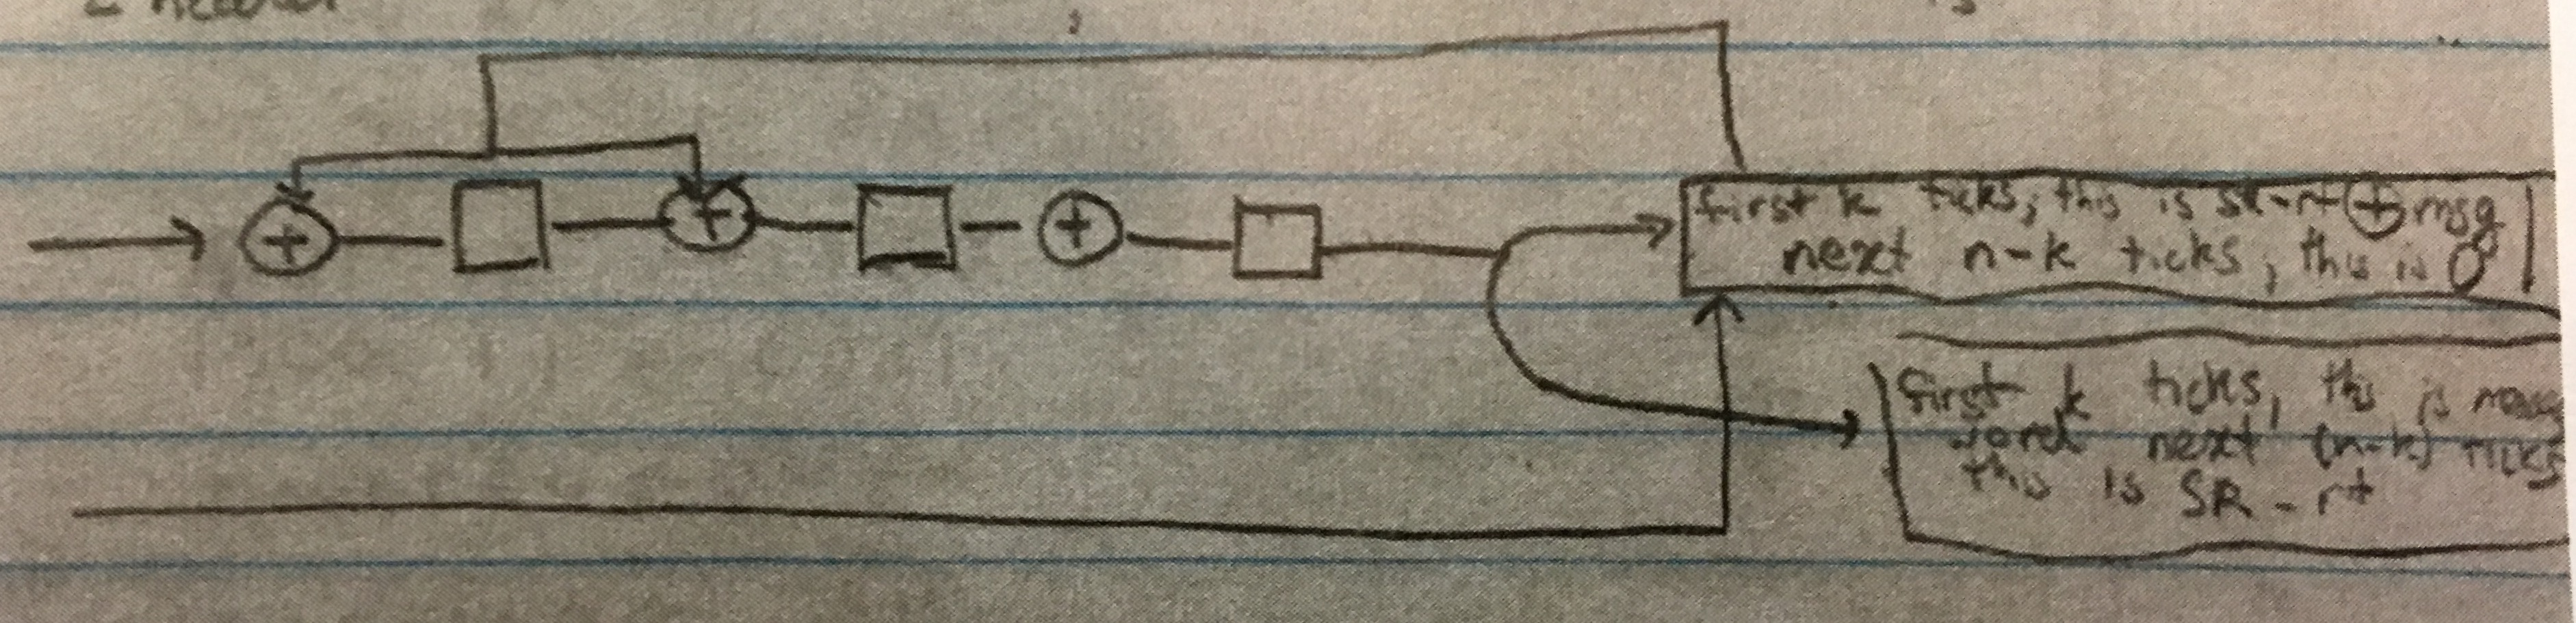
\includegraphics[width=\textwidth]{encoder.JPG}
\end{figure}

\noindent The resulting clock tick table is represented as follows:

\begin{figure}[ht]
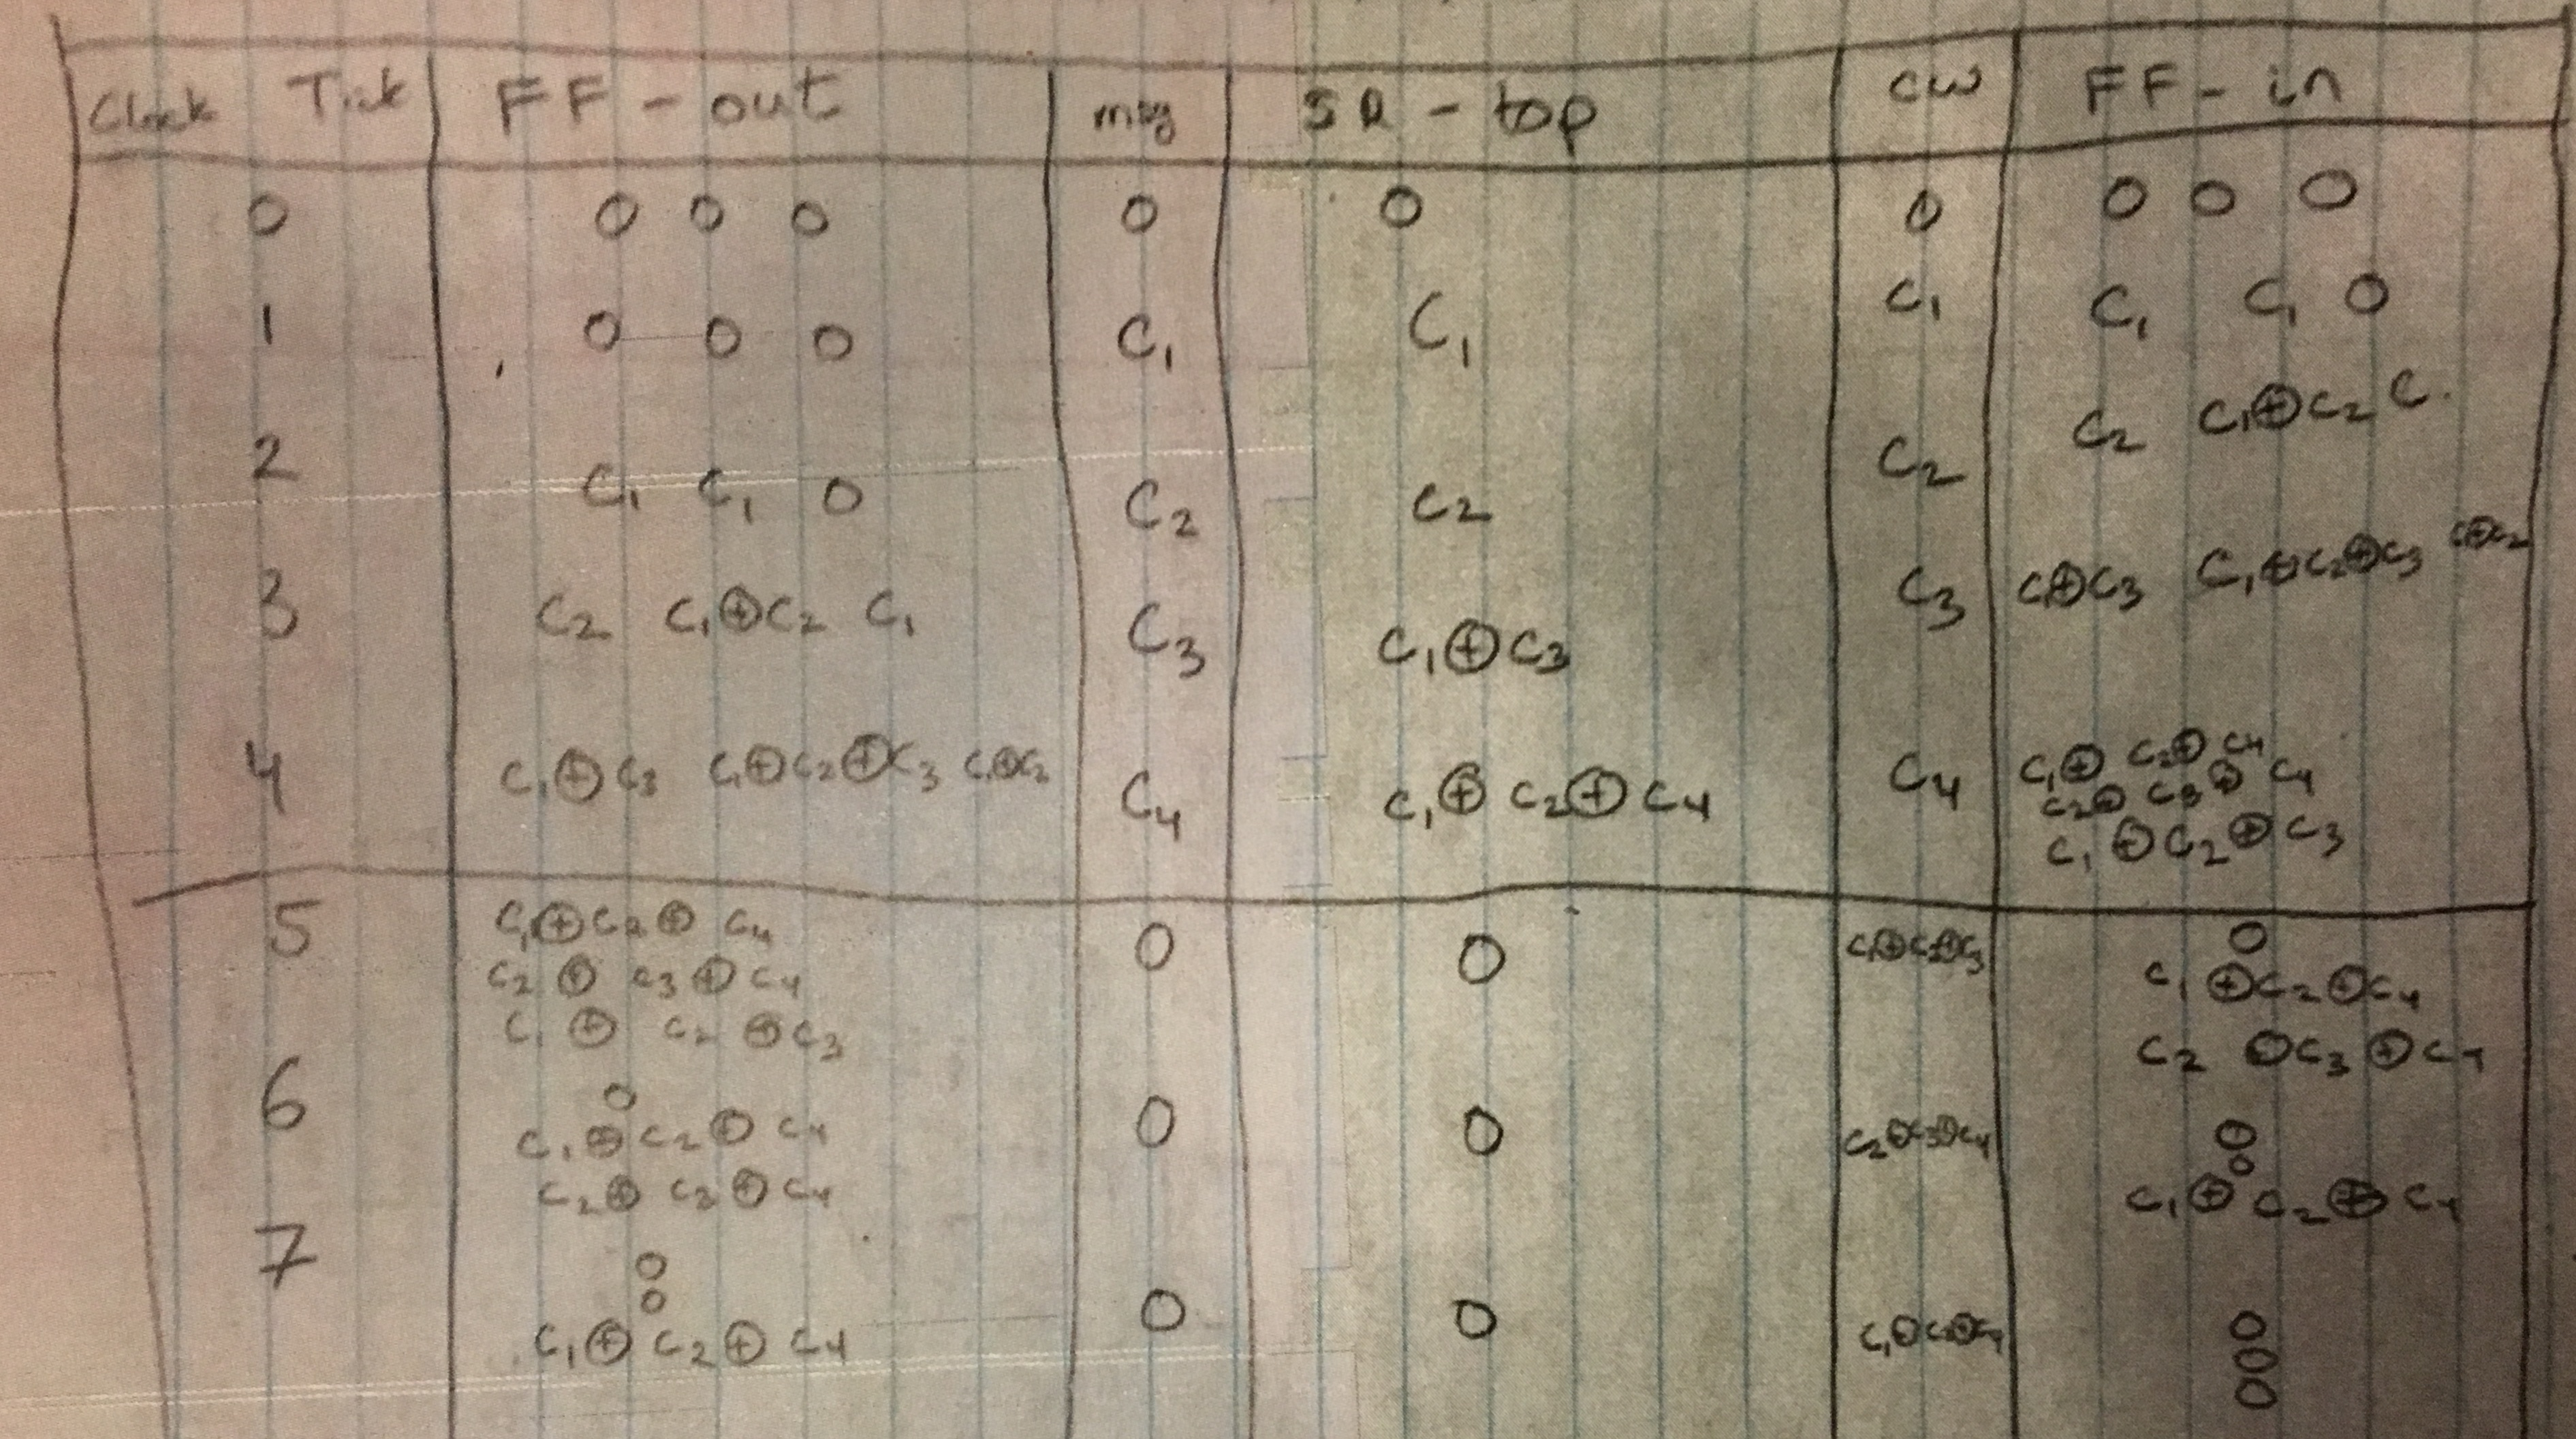
\includegraphics[width=\textwidth]{encoder2.JPG}
\end{figure}

\newpage
\subsubsection{Decoder Architecture}

For the first $n$ clock ticks, the received code word is input into the flip-flops, flushing out all previous zeros. The left input to SR (SR\_LFT) come exclusively from RCVD\_CW. For the next $n$ clock ticks, $n$ zeros are placed in the flip-flops. SR\_LFT is produced from the 101 detector output, and RCVD\_CW is output with all necessary corrections. The XOR without two inputs is--as before--simply a pass, and the 101 pattern is known as a syndrome. The decoder can be depicted by the following shift register sequence: 

\begin{figure}[ht]
\centering
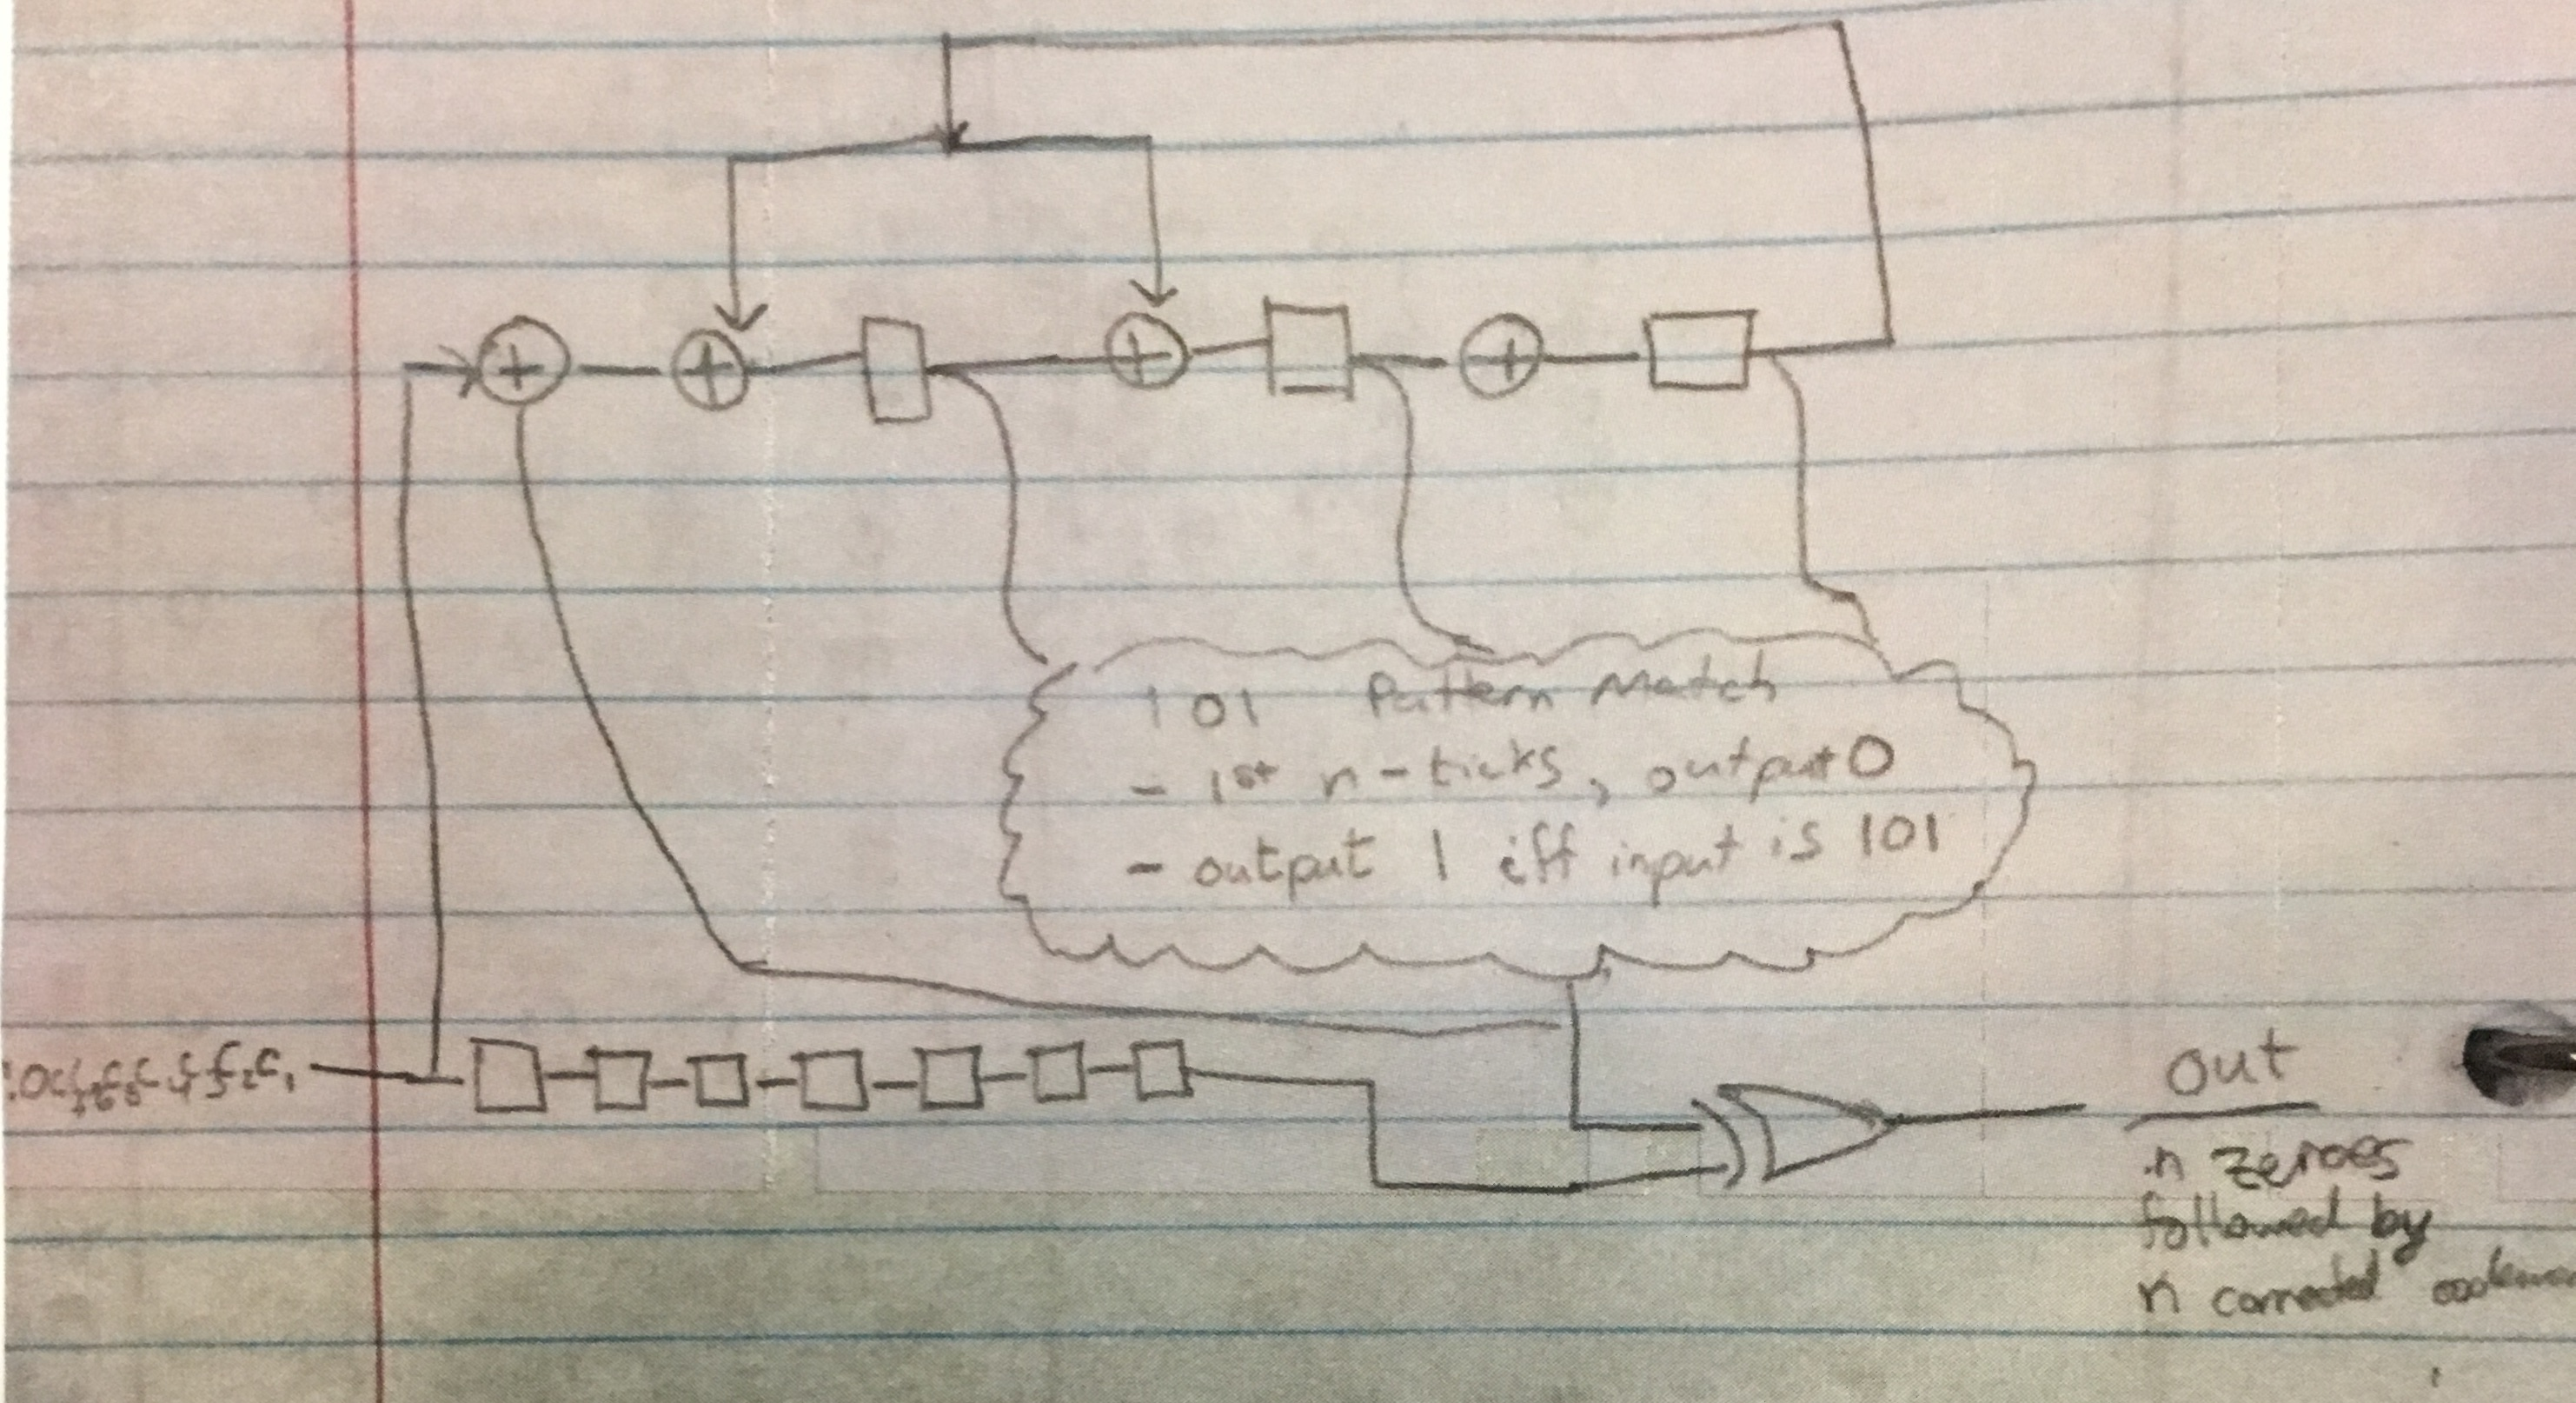
\includegraphics[width=.87\textwidth]{decoder.JPG}
\end{figure}

\noindent The resulting clock tick table is represented as follows:

\begin{figure}[ht]
\centering
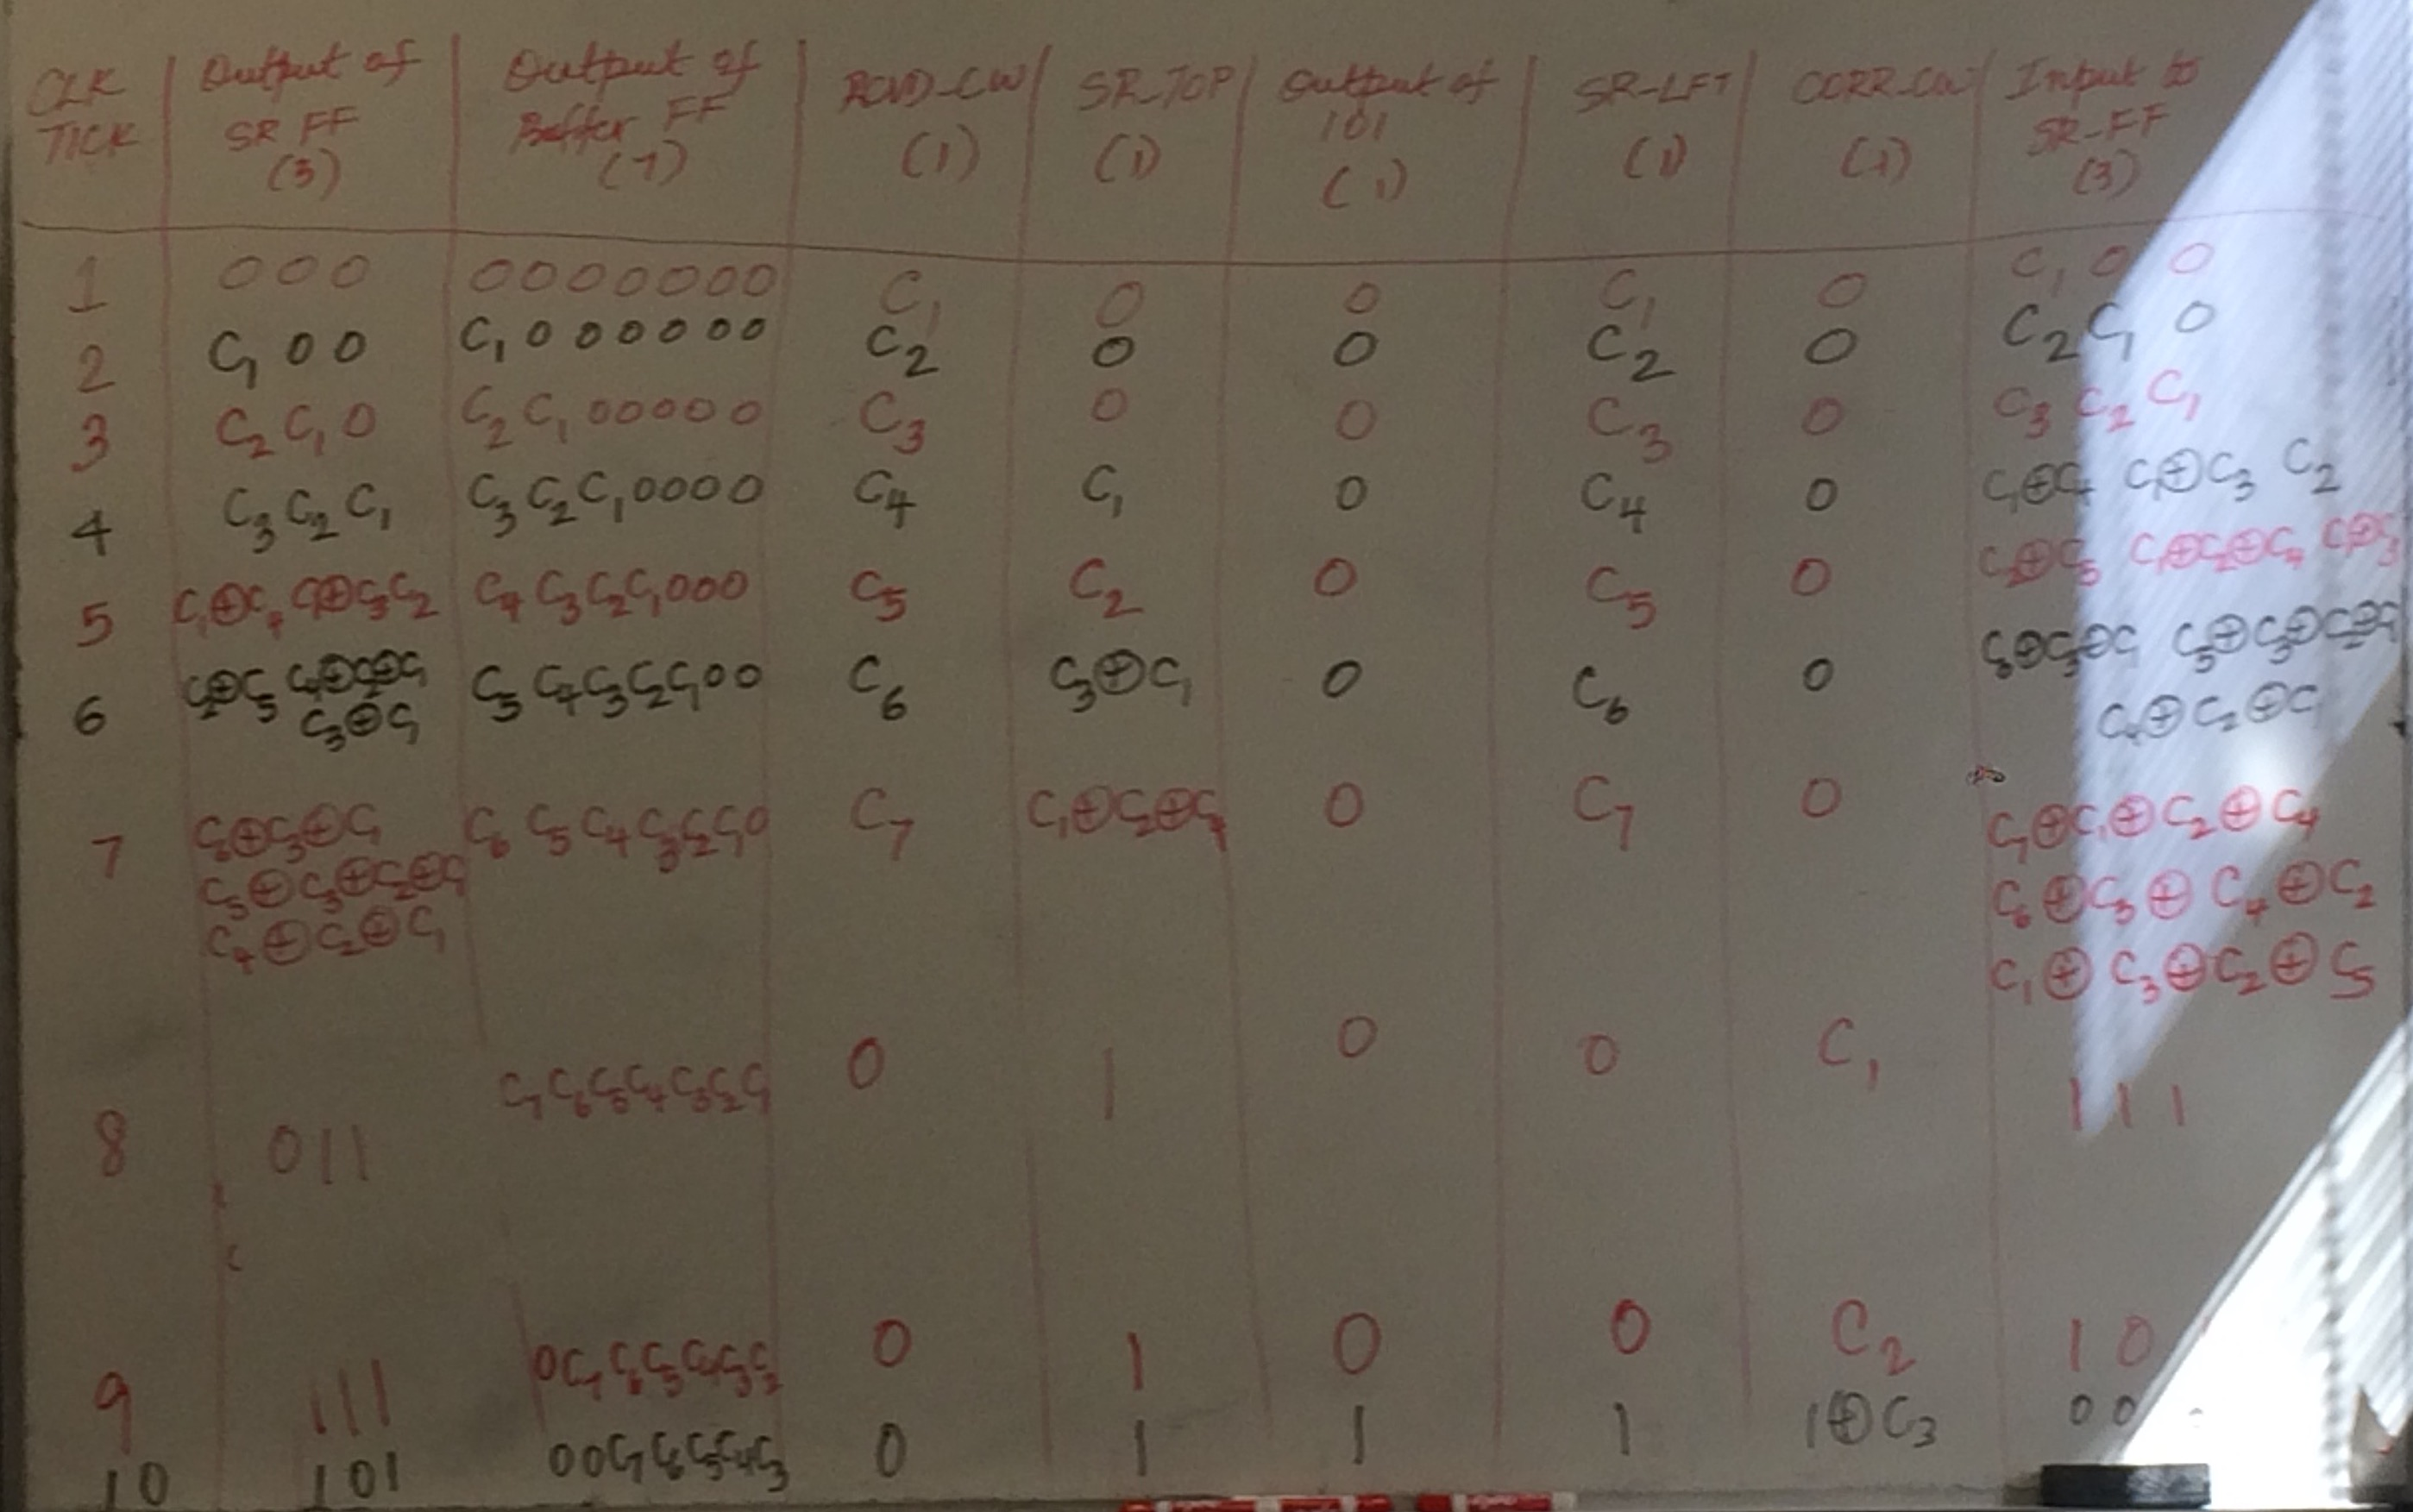
\includegraphics[width=.87\textwidth]{decoder2.JPG}
\end{figure}

\newpage
\section{December 5, 2016 (Andrew)}

\subsection{Channel Capacity Upper Bound}

Recall that $H(X)$ is a lower bound on the performance of any source encoder/decoder. 
$$\frac{\mathrm{avg. \, bits}}{\mathrm{src \, symbol}} \geq H(X)$$
On the channel side, 
$$\frac{\mathrm{avg. \, bits}}{\mathrm{ch. \, symbol}} \leq C(Y|X)$$

\subsection{Formulation for Proof of Upper Bound Theorem}
This proof will show that for a fixed channel with capacity $C(Y|X)$, the maximum amount of information that can be sent through that channel is bounded at a maximum of that capacity for all encoders and decoders.
\begin{enumerate}
	\item Pick a fixed channel with capacity $C(Y|X)$. 
	\item Pick any arbitrary channel encoder/decoder. 
	\item Assume that input bits to be transmitted are i.i.d. (Independent and Identically Distributed) 
	\item $P_{\mathrm{err}}$: Probability that a bit sent to the encoder is incorrectly read at decoder. This can be determined only with knowledge of the following:
		\begin{enumerate}
			\item How bits map to X
			\item What is $P(Y|X)$
			\item How Y maps to bits
		\end{enumerate}
	\item Part 1 of the Upper Bound Theorem says that $\frac{\mathrm{avg. \, bits}}{\mathrm{ch. \, symbol}} \leq \frac{C(Y|X) + H(P_{\mathrm{err}})}{1 - P_{\mathrm{err}}}$
	\item A ``Shannon family" of encoder/decoder pairs is an infinite sequence of encoder/decoder pairs $\{\langle E_i, D_i \rangle |i=1,2,3,...\}$ with $P_{\mathrm{err}} \rightarrow 0$. \\That is, $\forall \epsilon > 0, \exists \, i_0 \, \mathrm{s.t.} \, \forall i \geq i_0, P_{\mathrm{err}}(\langle E_i,D_i \rangle ) < \epsilon$\\
	{\bf Translated into English}: For all $\epsilon$ greater than zero, there exists an $i_0$ such that for all $i \geq i_0$, the probability of error for that encoder/decoder pair is less than $\epsilon$.\\
	{\bf Translated into Something Understandable}: Imagine a whole set of ways to map bits to channel codes and channel codes back to bits, these are your encoder/decoder pairs, $E_i$ and $D_i$. A ``Shannon family" is an infinite sequence of these pairs where the probability that an error is made in the encoding/decoding process approaches zero. In other words, given any threshold of error $\epsilon$, there will be some index in that sequence of encoder/decoder pairs such that that pair, $i_0$ and every following pair has a error rate less than or equal to epsilon. In short, it's a sequence of encoder/decoder pairs that have decreasing error rates that approach zero.  
	\item Take the limit of the family as $P_{\mathrm{err}} \rightarrow 0$.
\end{enumerate}
\subsection{Proof of Upper Bound Theorem}
\lemma {\bf Markov Lemma}. Given input bits $U$, input channel symbols $X$, output channel symbols $Y$, and output bits $V$, $I(U;V) \leq I(X;Y)$. Concretely, in the act of transmitting information across a channel, some of that information is lost. \\
{\bf Proof of the Lemma}: 
If A maps to B maps to C,
$$I(A;C) \leq I(B;C)$$
$$I(A;C) - I(B;C) \leq 0$$
\begin{align*}
	I(A;C) - I(B;C) 	&= E_{AC}\left[\log \left(\frac{P(C|A)}{P(C)} \right)\right] - E_{BC}\left[\log \left(\frac{P(C|B)}{P(C)} \right)\right]\\
				&= E_{ABC}\left[\log \left(\frac{P(C|A)}{P(C)} \right)\right] - E_{ABC}\left[\log \left(\frac{P(C|B)}{P(C)} \right)\right]\\
				&= E_{ABC}\left[\log \left(\frac{P(C|A)}{P(C|B)}\right) \right]\\
				&= \log \left(E_{ABC}\left[\frac{P(C|A)}{P(C|B)}\right]\right)\\
				&= \sum_{a,b,c} P(a,b,c) \frac{P(c|a)}{P(c|b)}\\
				&= \sum P(a) P(b|a) P(c|b)\\
				&= \sum P(a) P(b|a) P(c|a)\\
\end{align*}
The remainder of the proof is left as an exercise for the reader. We can see now that: 
$$I(A;C) \leq I(B;C)$$
$$I(A;C) \leq I(A;B)$$

\lemma {\bf Fano Lemma}. Given an input $U$ and an output $V$, 
$$H(U|V) \leq H(P_{\mathrm{err}}) + P_{\mathrm{err}} * H(U)$$
\\
{\bf From Lemma 1:}
$$I(U;V) \leq I(X;Y) \leq C(Y|X)$$
{\bf From Lemma 2:}
\begin{align*}
I(U;V) 	&= H(U) - H(U|V)\\
		&\geq H(U) - H(P_{\mathrm{err}}) + P_{\mathrm{err}} * H(U) \\
		&= (1 - P_{\mathrm{err}})H(U) - H(P_{\mathrm{err}})
\end{align*}
\\
{\bf Combining Lemmas 1 and 2:}
$$(1 - P_{\mathrm{err}})H(U) - H(P_{\mathrm{err}}) \leq C(Y|X)$$
$$H(U) \leq  \frac{C(Y|X) + H(P_{\mathrm{err}})}{1 - P_{\mathrm{err}}}$$
$$\frac{\mathrm{avg. \, bits}}{\mathrm{ch. \, symbol}} \leq \frac{C(Y|X) + H(P_{\mathrm{err}})}{1 - P_{\mathrm{err}}}$$
Taking the limit as $P_{\mathrm{err}}$ approaches zero:
\begin{align*}
	\lim_{P_{\mathrm{err}} \to 0} \frac{\mathrm{avg. \, bits}}{\mathrm{ch. \, symbol}} &= \lim_{P_{\mathrm{err}} \to 0} \frac{C(Y|X) + H(P_{\mathrm{err}})}{1 - P_{\mathrm{err}}}\\
	&= C(Y|X)
\end{align*}
\section{December 7, 2016: Putting it All Together (Andrew)}
\begin{table}[h]
	\begin{tabular}{|c|c|c|}
		\hline
		 Location & Theoretical Bound & Practically Possible \\
		 \hline
		 Source & $\frac{\mathrm{bits}}{\mathrm{src \, symbol}} \geq H(X)$ & $\frac{\mathrm{bits}}{\mathrm{src \, symbol}} \approx H(X)$ (e.g. Huffman)\\
		 \hline
		 Channel & $\frac{\mathrm{bits}}{\mathrm{ch \, symbol}} \leq C(Y|X)$ & $\frac{\mathrm{bits}}{\mathrm{ch \, symbol}} \approx C(Y|X)$ (no known algorithm)\\
		 \hline
	\end{tabular}
\end{table}

We define {\it reliable communication} as an encoder/decoder pair such that $P_{\mathrm{err}} \to 0$.

\theorem {\bf Shannon's Theorem:} Given any encoder/decoder pair and a channel for a source $X$, $P_{\mathrm{err}} \to 0$ if and only if $H(X) \leq C(Y|X)$. In other words, if channel capacity is greater than or equal to entropy, reliable communication is achievable.

\theorem {\bf Generalized Shannon's Theorem:} Given a source $X$ with average cost $\beta$ of sending information and a channel with average distortion $\delta$ on the received data, an encoder/decoder pair can be constructed such that $P_{\mathrm{err}} \to 0$ if and only if $H(X, \delta) \leq C(Y|X, \beta)$. In other words, if channel capacity at a given cost tolerance is greater than or equal to entropy at a given distortion tolerance, reliable communication is achievable.
 %----------
\newpage
\section*{Appendix A - Random Variables}
\begin{table}[h]
\centering
\begin{tabular}{|c|c|c|c|c|}
\hline
X & Pr[X=$x$] & E[X] & Var[X] & H[X] \\
\hline
Bernoulli & NA & $p$ & $p(1-p)$ & $-p\log{p} - (1-p)\log{(1-p)}$ \\
\hline
Binomial & $\binom{n}{k}p^{k}(1-p)^{n-k}$ & $np$ & $np(1-p)$ & NA \\
\hline
Geometric & $p(1 - p )^{k - 1}$ & $\frac{1}{p}$ & $\frac{1 - p}{p^2}$ & $\frac{-p\log{p} - (1-p)\log{(1-p)}}{p}$ \\
\hline
Poisson & $\frac{\lambda^k e^{-\lambda}}{k!}$ & $\lambda$ & $\lambda$ & NA \\
\hline
Uniform & $\frac{1}{b - a}$ & $\frac{1}{2}(a + b)$ & $\frac{1}{12}(b - a)^2$ & $\log{(b - a)}$\\
\hline
Exponential & $\lambda e^{-\lambda x}$ & $\frac{1}{\lambda}$ & $\frac{1}{\lambda^2}$   & $\log{\frac{e}{\lambda}}$ \\
\hline
Gaussian & $\frac{1}{\sqrt{2 \sigma^2 \pi}} e^{-\frac{(x - \mu)^2}{2 \sigma^2}}$ & $\mu$ & $\sigma^2$ & $\frac{1}{2}\log{2\pi e\sigma^2}$\\
\hline
\end{tabular}
\end{table}

\section*{Appendix B - Quotes}
\begin{itemize}
\item ``What's $p$, entropy?" (Shaya Zarkesh)
\item ``I can't do the math" (Swapnil Garg)
\item ``I still don't get it'' (Swapnil)
\item ``Swapnil---remember when, in 8th grade, I made JMO and you didn't?'' (Shaya) \\``I made USAMO.'' (Swapnil)
\item ``I'm just happy I'm not on the quotes page" (Neymika Jain)
\item ``How many fingers has a Martian?'' (Text)
\item ``2, 4, 6, 8, who do we appreciate? Not info theory!'' (Neymika)
\item ``I don't want to have as many [quotes] as Shaya...'' (Neymika)
\item ``So the entropy is bounded by $H[X]$ and $H[X] + 1$, right?'' (Manan Shah)
\item ``Isn't swapping kind of like gargling? Like you can put the code words in your mouth and gargle them...'' (Rose Guan)
\item ``Couldn't we make a pun with swapping and Swapnil?'' (Neymika)
\item ``This is Cauchy-Schwarz'' (Shaya) \\``No, it's just factoring'' (Kai Siang-Ang)\\``No, it's Cauchy'' (Shaya)\\``No, Shaya---No Cauchy, No Schwarz. Not related.'' (Dr. Aiyer)
\item ``I would be confused too if I actually understood what was happening'' (Neymika)
\item (Phone ringing) ``I guess it was mine'' (Dr. Aiyer) \\ ``Anu (I knew) it was yours!'' (Shaya)
\item ``Time flies when you're... proving things'' (Manan)
\item ``So Justin, what's the answer?'' (Dr. Aiyer) \\ ``7'' (Justin Jia) \\ ``Wrong, because you didn't phrase it in the form of a question.'' (Dr. Aiyer)
\item ``Um, Dr. Aiyer, are we going to go over the PSAT math thing in class?'' (Rose)
\item ``So what's 0.85 + 0.3?'' (Neymika)
\item ``What are we supposed to be doing right now?'' (Swapnil) (and variations on a theme, x16)
\item ``So are you going to talk through it or do it?'' (Dr. Aiyer) \\ ``Oh, I don't really know how to do it...'' (Swapnil)
\item ``So how does stuff start cancelling out'' (Justin)
\item ``No, you can't be clever, that's not allowed in this class.'' (Dr. Aiyer)
\item ``We could actually get this with algebra if we were clever enough, but we’re not clever enough.'' (Rajiv Movva)
\item ``So how long did the homework take you?" (Shaya) \\ ``About fifty minutes" (Swapnil) \\ ``Yeah it took me about fifty minutes too" (Shaya) \\ ``It took you \textit{fifty} minutes?" (Swapnil) \\ ``It took you fifty minutes too..." (Shaya) \\ ``No, but it took \textit{you} fifty minutes" (Swapnil)
\item ``Prepare to have your mind blown...'' \\ ``...wait, shit.'' (Shaya)
\item ``He's going to include the s-h-i-t word'' (Neymika)
\item ``Wait, what do you mean no computation? Do you \textit{suppress} all computation?'' (Swapnil) \\ (5 minutes later) ``I don't know how to intuit this...'' (Shaya) \\ ``Yeah, I accidentally computed.'' (Swapnil)
\item ``We have to de-jiggle the input'' (Andrew Tierno) 
\item ``This will all make sense, right?'' (Neymika) 
\item ``Randy, just do it on the board and I'll correct you.'' (Swapnil)
\item ``2 times 3 is 6 times 4 is 8'' (Shaya)
\item ``Oxford English Dictionary...there has to be something wrong with that right from the name.'' (Dr. Aiyer)
\item ``What does the noise look like?'' (Steven Cao) \\ ``Probably Gaussian.'' (Rajiv)
\item ``Capacity sounds like rate'' (Shaya) \\ ``Why?'' (Everyone) \\ ``They both have `A's'' (Shaya)
\item ``It's uncountably finite...wait, no, it's countably infinite'' (Manan)
\item ``You have to actually \textit{think} about the problem, Shaya'' (Swapnil)
\item ``Our idea is better.'' (Manan) \\ ``On what grounds?'' (Dr. Aiyer) \\ ``It uses more flip-flops!'' (Rose)
\item ``But like, how does that work with wires?'' (Shaya)
\item ``That's just my notation, I defined it that way'' (Steven Cao)
\item ``Woah." (Swapnil)
\end{itemize}
\end{document}
